\documentclass[tikz, tcolorbox]{summary}
%=================================================================
\title{Summary}
\headtitle{AIRCRAFTS -- SUMMARY}
\author{PBREUER}

% Undefine \imath and \jmath to avoid conflict between breqn and sfmath
\let\imath\relax
\let\jmath\relax
% sfmath also redefines \ldotp, so relax it before loading the package
\let\ldotp\relax
% sfmath redefines uppercase Greek letters; relax them to avoid duplicate definitions
\let\Gamma\relax
\let\Delta\relax
\let\Theta\relax
\let\Lambda\relax
\let\Xi\relax
\let\Pi\relax
\let\Sigma\relax
\let\Upsilon\relax
\let\Phi\relax
\let\Psi\relax
\let\Omega\relax
\usepackage[cmbright]{sfmath}

\usepackage{algpseudocode} % pseudocode

\begin{document}

	% restart page counter
	\setcounter{page}{1}
	% reactivate header and footer
	\pagestyle{plain}

	\begin{multicols*}{3}
		\LARGE \textbf{\colorbox{black}{\textcolor{white}{AIRCRAFT AERODYNAMICS}}} \\
		\normalsize 
        %\textbf{\colorbox{color2}{\textcolor{white}{\url{URL}}}} \\
        \textbf{\colorbox{color2}{\textcolor{white}{\href{mailto:pbreuer@ethz.ch}{PBREUER}}}}
        \blue{Rev: \today}
        \normalsize

	\section{AERODYNAMIC FORCES}

\begin{whitebox}{}
    \begin{tabularx}{\columnwidth}{lclclc}
        $L$ & $\unit{N}$ & Lift force\\
        $D$ & $\unit{N}$ & Drag force\\
        $V$ & $\unit{m.s^{-1}}$ & Velocity\\
        $\rho$ & $\unit{kg.m^{-3}}$ & Air density\\
        $S_{ref}$ & $\unit{m^2}$ & Wing reference area\\
        $c_L$ & $-$ & Lift coefficient\\
        $c_D$ & $-$ & Drag coefficient\\
        $c_{D0}$ & $-$ & Zero-lift drag coefficient\\
        $c_{Di}$ & $-$ & Induced drag coefficient\\
        $k$ & $-$ & $k$-Factor\\
        $AR$ & $-$ & Aspect ratio\\
        $e$ & $-$ & Oswald efficiency factor & $\in[0,1]$\\
    \end{tabularx}
\end{whitebox}


\begin{highlightbox}{\textbf{LIFT \& DRAG}}
    \begin{align}
        \label{eq:lift}
        &L=\frac{1}{2}\rho V^2S_{ref}c_L\\
        \label{eq:drag}
        &D=\frac{1}{2}\rho V^2S_{ref}c_D
    \end{align}
\end{highlightbox}

\begin{highlightbox}{\textbf{QUADRATIC DRAG MODEL}}
    \begin{align}
        \label{eq:drag_coeff}
        &c_D=c_{D0}+c_{Di}\\
        \label{eq:ind_drag_coeff}
        &c_{Di}=kc_L^2\\
        \label{eq:k_factor}
        &k=\frac{1}{\pi ARe}
    \end{align}
\end{highlightbox}


	\section{2D EQUATIONS OF MOTION}

\begin{whitebox}{}
    \begin{tabularx}{\columnwidth}{lclclc}
        $T$ & $\unit{N}$ & Thrust force\\
        $m$ & $\unit{kg}$ & Mass\\
        $g$ & $\unit{m.s^{-2}}$ & Gravitational accel. & $9.80665\ \unit{m.s^{-2}}$\\
        $\gamma$ & $\unit{rad}$ & Flight path angle\\
        %$\bar{\gamma}$ & $\unit{rad}$ & Glide angle\\
        $\alpha$ & $\unit{rad}$ & Angle of attack\\
        $\sigma$ & $\unit{rad}$ & Thrust incidence angle\\
        $V_C$ & $\unit{m.s^{-1}}$ & Climb speed\\
        $V_S$ & $\unit{m.s^{-1}}$ & Sink speed\\
        $V_H$ & $\unit{m.s^{-1}}$ & Horizontal speed\\
    \end{tabularx}
\end{whitebox}

\resizebox{1.0\linewidth}{!}{
    \includegraphics[
    page = {14},
    trim = {6.0cm, 7.7cm, 6.0cm, 3.8cm}, % left, bottom, right, top
    clip
    ]{Lecture01.pdf}
}

\begin{highlightbox}{\textbf{GENERAL 2D EQUATIONS OF MOTION}}
    \begin{align}
        \label{eq:2d_eom_x}
        (x) \quad &m\dot{V}=T\cos(\alpha+\sigma)-D-mg\sin\gamma\\
        \label{eq:2d_eom_y}
        (y) \quad &mV\dot{\gamma}=L+T\sin(\alpha+\sigma)-mg\cos\gamma
    \end{align}
\end{highlightbox}

\begin{highlightbox}{\textbf{HORIZONTAL \& VERTICAL SPEED}}
    \begin{align}
        \label{eq:2d_eom_horizspeed}
        &V_H=V\cos\gamma\\
        \label{eq:2d_eom_vertspeed}
        &V_C=V_S=V\sin\gamma
    \end{align}
\end{highlightbox}

\begin{whitebox}{\textbf{STATIONARY GLIDING FLIGHT}}
    \blue{Conditions}
    \begin{itemize}
        \item $T=0$
        \item $\sfrac{d(\cdot)}{dt}=0$
    \end{itemize}
    
    \blue{Assumptions}
    \begin{itemize}
        \item $\alpha\approx 0$
        \item $\sigma\approx0$
    \end{itemize}
    
    \begin{highlightbox}{}
        \begin{align}
            \label{eq:stat_glide_drag}
            &D=mg\sin\gamma\\
            \label{eq:stat_glide_lift}
            &L=mg\cos\gamma
        \end{align}
    \end{highlightbox}

    \centering
    \resizebox{0.6\linewidth}{!}{
        \includegraphics[
        page = {25},
        trim = {10.5cm, 1.0cm, 4.5cm, 8.5cm}, % left, bottom, right, top
        clip
        ]{Lecture01.pdf}
    }
    \resizebox{1.0\linewidth}{!}{
        \includegraphics[
        page = {28},
        trim = {1.0cm, 5.5cm, 6.5cm, 2.5cm}, % left, bottom, right, top
        clip
        ]{Lecture01.pdf}
    }

    \mathbox{
        \frac{V_H}{V_S}=\frac{L}{D}\overset{\scriptscriptstyle\eqref{eq:lift},\eqref{eq:drag}}{=}\frac{c_L}{c_D}=\frac{1}{\tan\gamma}\overset{\gamma\ll1}{\approx}\frac{1}{\gamma}
    }
    
    \mathbox{
        \tan(\gamma_{\min})=\frac{1}{\left(\frac{c_L}{c_D}\right)_{\max}}
    }
    
    \mathbox{
        V\overset{\scriptscriptstyle\eqref{eq:lift}}{=}\sqrt{\frac{2mg}{\rho S_{ref}c_L}\cos\gamma}\overset{\gamma\ll1}{\approx}\sqrt{\frac{2mg}{\rho S_{ref}c_L}}
    }
    
    \mathbox{
        V_S=\sqrt{\frac{2mg}{\rho S_{ref}}\frac{c_D^2}{c_L^3}\cos^3(\gamma)} \overset{\gamma\ll1}{\approx}\sqrt{\frac{2mg}{\rho S_{ref}}\frac{c_D^2}{c_L^3}}
    }
    
    \mathbox{
        V_H=\sqrt{V^2-V_S^2}
    }
    
    \mathbox{
        V_{H,\min}\overset{\gamma\ll1}{\approx}V(c_L=c_{L,\max})
    }
    
    \mathbox{
        V_{S,\min}\overset{\gamma\ll1}{\approx}V_S\left(\left(\frac{c_L^3}{c_D^2}\right)_{\max}\right)
    }

\end{whitebox}

        \section{PROPULSION}

\resizebox{1.0\linewidth}{!}{
    \includegraphics[
    page = {5},
    trim = {2.0cm, 5.0cm, 2.0cm, 3.5cm}, % left, bottom, right, top
    clip
    ]{Lecture03.pdf}
}

\begin{whitebox}{}
    \begin{tabularx}{\columnwidth}{lclclc}
        $\dot{m}$ & $\unit{kg.s^{-1}}$ & Air flow\\
        $V_\infty$ / $V_0$ & $\unit{m.s^{-1}}$ & Freestream velocity\\
        $p_\infty$ & $\unit{Pa}$ & Freestream pressure\\
        $V_e$ / $V_3$ & $\unit{m.s^{-1}}$ & Exit velocity\\
        $p_e$ & $\unit{Pa}$ & Exit pressure\\
        $A_i$ & $\unit{m^2}$ & Inlet area\\
        $A_e$ & $\unit{m^2}$ & Exit area\\
        $\eta_{tot}$ & $-$ & Total efficiency\\
        $\eta_t$ & $-$ & Thermal efficiency\\
        $\eta_p$ & $-$ & Propulsive efficiency\\
        $P_{m}$ & $\unit{W}$ & Engine mechanical output power\\
        $\dot{m}_f$ & $\unit{kg.s^{-1}}$ & Fuel flow\\
        $HV$ & $\unit{J.kg^{-1}}$ & Fuel heating value\\
        $T_{avail}$ & $\unit{N}$ & Available thrust\\
        $P_{avail}$ & $\unit{W}$ & Available power\\
        $T_c$ & $-$ & Thrust coefficient\\
        $A$ & $\unit{m^2}$ & Propeller disc area\\
        $\eta_i$ & $-$ & Propeller efficiency\\
        $w$ & $\unit{m.s^{-1}}$ & Velocity induced at propeller\\
        $V_1$ & $\unit{m.s^{-1}}$ & Velocity at propeller disc\\
    \end{tabularx}
\end{whitebox}

\begin{whitebox}{\textbf{THRUST}}
    \resizebox{1.0\linewidth}{!}{
    \includegraphics[
    page = {6},
    trim = {12.0cm, 12.0cm, 2.0cm, 2.5cm}, % left, bottom, right, top
    clip
    ]{Lecture03.pdf}
    }
    \begin{highlightbox}{MOMENTUM}
        \textbf{Note} Control surface $CS$
        \begin{align}
            \label{eq:thrust_momentum}
            F_x=\oiint_{C S} V_x(\rho\vec{V}\cdot d\vec{A})=-\rho_{\infty} V_{\infty} V_{\infty} A_i+\rho_e V_e V_e A_e
        \end{align}
    \end{highlightbox}
    \begin{highlightbox}{CONTINUITY}
        \begin{align}
            \label{eq:thrust_continuity}
            \dot{m}=\rho_{\infty} V_{\infty} A_i=\rho_e V_e A_e=\text {const.}
        \end{align}
    \end{highlightbox}
    \begin{highlightbox}{EXTERNAL FORCES}
        \begin{align}
            \label{eq:thrust_ext_forces}
            F_x=T-(p_e-p_\infty)A_e
        \end{align}
    \end{highlightbox}
    \begin{highlightbox}{EFFICIENCY}
        \begin{align}
            \label{eq:thrust_total_efficiency}
            &\eta_{t o t}=\frac{T V}{\dot{m}_f H V}=\eta_t \eta_p\\
            \label{eq:thrust_thermal_efficiency}
            &\eta_t=\frac{P_m}{\dot{m}_f H V}\\
            \label{eq:thrust_propulsive_efficiency}
            &\eta_p=\frac{T V}{P_m}
        \end{align}
    \end{highlightbox}

    \mathbox{
        F_x=-\dot{m}V_\infty+\dot{m}V_e
    }
    \mathbox{
        &T=\dot{m}(V_e-V_\infty)+(p_e-p_\infty)A_e\\
        &\overset{p_e-p_\infty\approx 0}{\approx}\dot{m}(V_e-V_\infty)
    }
\end{whitebox}

\begin{whitebox}{\textbf{ACTUATOR DISC THEORY}}
    \blue{Assumptions}
    \begin{itemize}
        \item Incompressible i.e. $\rho=$ const.
        \item $V_1=$ const.
        \item Uniform pressure over disc
        \item No rotational effects
    \end{itemize}
    \centering
    \resizebox{0.7\linewidth}{!}{
    \includegraphics[
    page = {11},
    trim = {12.0cm, 6.0cm, 0.5cm, 2.5cm}, % left, bottom, right, top
    clip
    ]{Lecture03.pdf}
    }
    \begin{highlightbox}{THRUST}
        \begin{align*}
            T=A(p_2-p_1)
        \end{align*}
    \end{highlightbox}
    \begin{highlightbox}{POWER}
        \begin{align*}
            P=2\rho Aw(V_0+w)^2
        \end{align*}
    \end{highlightbox}
    \begin{highlightbox}{THRUST COEFFICIENT}
        \begin{align*}
            T_c=\frac{T}{\frac{1}{2}\rho V_0^2A}
        \end{align*}
    \end{highlightbox}
        \begin{highlightbox}{BERNOULLI'S EQUATION}
        \begin{align*}
            p+\frac{1}{2}\rho V^2+\rho gh=\text{const.}
        \end{align*}
    \end{highlightbox}
    \mathbox{
        T\overset{\scriptscriptstyle\eqref{eq:thrust_momentum},\eqref{eq:thrust_continuity}}{=}\rho AV_1(V_3-V_0)
    }
    \mathbox{
        T=\frac{\rho}{2}A(V_3^2-V_0^2)
    }
    \mathbox{
        &V_1=\frac{V_3+V_0}{2}=V_0+w\\
        &V_3=2V_1-V_0=V_0+2w
    }
    \mathbox{
        T=\rho A(V_0+w)\cdot 2w
    }
    \mathbox{
        &P=T(V_0+w)\\
        &P_{use}=TV_0\\
        &P_{ind}=Tw
    }
    \mathbox{
        w=-\frac{V_0}{2}+\sqrt{\left(\frac{V_0}{2}\right)^2+\frac{1}{2 \rho} \frac{T}{A}}
    }
    \mathbox{
        \eta_i=\frac{P_{use}}{P}=\frac{2}{1+\sqrt{1+T_c}}
    }
\end{whitebox}

\begin{whitebox}{\textbf{TURBOJET MODEL}}
    \blue{Assumptions}
    \begin{itemize}
        \item $T_{avail}=$ const.
    \end{itemize}
\end{whitebox}

\begin{whitebox}{\textbf{TURBOPROP MODEL}}
    \blue{Assumptions}
    \begin{itemize}
        \item $P_{avail}=$ const.
    \end{itemize}
\end{whitebox}

\begin{highlightbox}{\textbf{POWER}}
    \begin{align*}
        P_{avail}=T_{avail}V
    \end{align*}
\end{highlightbox}


        \section{SPECIFIC EXCESS POWER}

\begin{whitebox}{}
    \begin{tabularx}{\columnwidth}{lclclc}
        $E$ & $\unit{J}$ & Total energy\\
        $E_p$ & $\unit{J}$ & Potential energy\\
        $E_k$ & $\unit{J}$ & Kinetic energy\\
        $h$ & $\unit{m}$ & Height above ground\\
        $h_e$ / $E_s$ & $\unit{m}$ & Specific energy / energy height\\
        $SEP$ / $P_s$ & $\unit{m.s^{-1}}$ & Specific excess power
    \end{tabularx}
\end{whitebox}

\begin{highlightbox}{}
    \begin{align*}
        &E=E_p+E_k=mgh+\frac{1}{2}mV^2\\
        &h_e=E_s=\frac{E}{mg}=h+\frac{V^2}{2g}\\
        &SEP=P_s=\frac{dh_e}{dt}=V_C+\frac{V}{g}\frac{dV}{dt}
    \end{align*}
\end{highlightbox}

        \section{CRUISE PERFORMANCE}

\begin{whitebox}{}
    \begin{tabularx}{\columnwidth}{lclclc}
        $T_{req}$ & $\unit{W}$ & Required power\\
    \end{tabularx}
\end{whitebox}

\begin{whitebox}{\textbf{STATIONARY LEVEL CRUISE FLIGHT}}
    \blue{Conditions}
    \begin{itemize}
        \item $\gamma=0$
        \item $\sfrac{d(\cdot)}{dt}=0$
    \end{itemize}
    
    \blue{Assumptions}
    \begin{itemize}
        \item $\alpha\approx0$
        \item $\sigma\approx0$
    \end{itemize}
    
    \begin{highlightbox}{}
    \begin{align}
        \label{eq:stat_cruise_thrust}
        &T=D\\
        \label{eq:stat_cruise_lift}
        &L=mg
    \end{align}
    \end{highlightbox}

    \mathbox{
        D\overset{\scriptscriptstyle\eqref{eq:lift},\eqref{eq:drag},\eqref{eq:drag_coeff},\eqref{eq:ind_drag_coeff}}{=}\frac{1}{2}\rho V^2S_{ref}c_{D0}+k\cdot\frac{(mg)^2}{\frac{1}{2}\rho V^2S_{ref}}=T_{req}
    }
    \resizebox{1.0\linewidth}{!}{
        \includegraphics[
            trim = {0.0cm, 0.0cm, 1.0cm, 0.0cm}, % left, bottom, right, top
            clip
            ]{Graph_Drag_Bucket.pdf}
    }
    \resizebox{1.0\linewidth}{!}{
        \includegraphics[
            trim = {0.0cm, 0.0cm, 1.0cm, 0.0cm}, % left, bottom, right, top
            clip
            ]{Graph_Max_Cruise.pdf}
    }
\end{whitebox}



        \section{CLIMB PERFORMANCE}

\begin{whitebox}{}
    \begin{tabularx}{\columnwidth}{lclclc}
        $V_{C,SL}$ & $\unit{m.s^{-1}}$ & Climb speed at sea level\\
        $h_{ceil}$ & $\unit{m}$ & Absolute ceiling\\
        $t_C$ & $-$ & Time to climb\\
        $P_{req}$ & $\unit{W}$ & Required power
    \end{tabularx}
\end{whitebox}

%\begin{whitebox}{}
%    \begin{tabularx}{\columnwidth}{lclclc}
%        $T$ & $\unit{N}$ & Thrust\\
%        $m$ & $\unit{kg}$ & Mass\\
%    \end{tabularx}
%\end{whitebox}

\begin{whitebox}{\textbf{STATIONARY CLIMB}}
    \blue{Conditions}
    \begin{itemize}
        \item $\sfrac{d(\cdot)}{dt}=0$
    \end{itemize}
    
    \blue{Assumptions}
    \begin{itemize}
        \item $\alpha\approx0$
        \item $\sigma\approx0$
    \end{itemize}

    \begin{highlightbox}{}
    \begin{align*}
        &T=D+mg\sin\gamma\\
        &L=mg\cos\gamma
    \end{align*}
    \end{highlightbox}
    
    \mathbox{
        P_s\overset{\scriptscriptstyle\eqref{eq:2d_eom_x},\eqref{eq:2d_eom_vertspeed}}{=}V\frac{T\cos(\alpha+\sigma)-D}{mg}\overset{\alpha+\sigma\ll1}{\approx}V\cdot\frac{T-D}{mg}
    }
    \mathbox{
        &P_{avail}=TV\\
        &P_{req}=DV\\
        &P_S\overset{\alpha+\sigma\ll1}{\approx}\frac{P_{avail}-P_{req}}{mg}
    }
    \mathbox{
        V_{C,max}=P_{s,max}
    }   
    \textbf{Note} Simplify calculation of $D$ by assuming \eqref{eq:stat_cruise_lift} i.e. $\gamma=0$

    \begin{center}
        \resizebox{0.8\linewidth}{!}{
            \includegraphics[
            page = {10},
            trim = {1.2cm, 6.2cm, 11.0cm, 6.0cm}, % left, bottom, right, top
            clip
            ]{Lecture02.pdf}
        }        
    \end{center}

    \resizebox{1.0\linewidth}{!}{
        \includegraphics[
        trim = {0.0cm, 0.0cm, 1.0cm, 0.0cm}, % left, bottom, right, top
        clip
        ]{Graph_SEP.pdf}
    }

    \begin{highlightbox}{CEILINGS}
        \begin{align*}
            V_C(h)=V_{C,SL}\left(1-\frac{h}{h_{ceil}}\right)
        \end{align*}
    \end{highlightbox}
    
    \resizebox{0.9\linewidth}{!}{
        \includegraphics[
        trim = {0.0cm, 0.0cm, 1.0cm, 0.0cm}, % left, bottom, right, top
        clip
        ]{Graph_Ceilings.pdf}
    }

    \blue{Assumptions}
    \begin{itemize}
        \item $V_C=V_C(h)$
    \end{itemize}
    \begin{highlightbox}{TIME TO CLIMB}
        \begin{align*}
            &t_C=\int_{h_0}^{h_1} \frac{1}{V_C(h)} d h=\ldots=\frac{1}{V_{C, S L}} \cdot \ln \left(\frac{1}{1-\frac{h}{h_{c e i l}}}\right)
        \end{align*}
    \end{highlightbox}
\end{whitebox}


        \vfill\null 
        \columnbreak

        \section{TAKEOFF PERFORMANCE}

\begin{whitebox}{}
    \begin{tabularx}{\columnwidth}{lclclc}
        $V_{stall}$ & $\unit{m.s^{-1}}$ & Stall speed\\
        $V_1$ & $\unit{m.s^{-1}}$ & Decision speed\\
        $V_R$ & $\unit{m.s^{-1}}$ & Rotation speed\\
        $V_{mu}$ & $\unit{m.s^{-1}}$ & Minimum unstick speed\\
        $V_{LOF}$ & $\unit{m.s^{-1}}$ & Liftoff speed\\
        $V_2$ & $\unit{m.s^{-1}}$ & Takeoff safety speed\\
        $h_{obs}$ & $\unit{m}$ & Obstacle height\\
        $\mu$ & $-$ & Ground friction coefficient\\
        $t_R$ & $\unit{s}$ & Time to takeoff\\
        $s_R$ & $\unit{s}$ & Distance to takeoff\\
        $\alpha_{tailstrike}$ & $\unit{rad}$ & Angle of attack causing tailstrike\\
        $\alpha_{\max}$ & $\unit{rad}$ & Angle of attack corresponding to $c_{L,\max}$\\
        $c_{D i,IGE}$ & $-$ & Induced drag coefficient in ground effect
    \end{tabularx}
\end{whitebox}

\resizebox{0.9\linewidth}{!}{
    \includegraphics[
    page = {25},
    trim = {1.5cm, 8.0cm, 3.5cm, 2.5cm}, % left, bottom, right, top
    clip
    ]{Lecture02.pdf}
}

\resizebox{0.9\linewidth}{!}{
    \includegraphics[
    page = {21},
    trim = {1.8cm, 5.0cm, 1.0cm, 8.0cm}, % left, bottom, right, top
    clip
    ]{Lecture02.pdf}
}

\begin{highlightbox}{\textbf{GROUND ROLL}}
    \begin{align*}
        &T-D-\mu(mg-L)=F_{res}=m\frac{dV}{dt}\\
        &t_R=\int_0^{t_R} d t=m \int_0^{V_{L O F}} \frac{1}{F_{r e s}} d V\\
        &s_R=\int_0^{t_R} V d t=m \int_0^{V_{L O F}} \frac{V}{F_{\text {res }}} d V
    \end{align*}
\end{highlightbox}


\begin{whitebox}{\textbf{TAILSTRIKE}}
    \blue{Assumptions}
    \begin{itemize}
        \item $\alpha_{tailstrike}<\alpha_{max}$
        \item $c_{L,mu}<c_{L,max}$
    \end{itemize}
    \begin{highlightbox}{}
        \begin{align*}
            &V_{m u}=\sqrt{\frac{2 m g}{\rho S_{r e f} c_{L, m u}}}>V_{stall}=\sqrt{\frac{2 m g}{\rho S_{r e f} c_{L, \max }}}
        \end{align*}
    \end{highlightbox}
\end{whitebox}

\begin{whitebox}{\textbf{GROUND EFFECT}}
    \blue{Conditions}
    \begin{itemize}
        \item $h\leq\sfrac{1}{2}$ wingspan
    \end{itemize}
    
    \begin{highlightbox}{}
        \begin{align*}
            \frac{c_{D i,IGE}}{c_{D i}}=\frac{\left(16 \frac{h}{b}\right)^2}{1+\left(16 \frac{h}{b}\right)^2}
        \end{align*}
    \end{highlightbox}
\end{whitebox}

        \section{LANDING PHASE}

\begin{whitebox}{}
    \begin{tabularx}{\columnwidth}{lclclc}
        $V_{APP}$ & $\unit{m.s^{-1}}$ & Approach speed\\
        $\gamma_{APP}$ & $\unit{rad}$ & Approach flight path angle\\
    \end{tabularx}
\end{whitebox}

\resizebox{1.0\linewidth}{!}{
    \includegraphics[
    page = {3},
    trim = {2.0cm, 1.0cm, 2.0cm, 10.0cm}, % left, bottom, right, top
    clip
    ]{Lecture03.pdf}
}

        \vfill\null 
        \columnbreak

        \section{MANEUVER PERFORMANCE}

\begin{whitebox}{}
    \begin{tabularx}{\columnwidth}{lclclc}
        $a_n$ & $\unit{m.s^{-2}}$ & Centripetal acceleration\\
        $r$ & $\unit{m}$ & Turn radius\\
        $\Psi$ & $\unit{rad}$ & Turn angle\\
        $\dot{\Psi}$ & $\unit{rad.s^{-1}}$ & Turn rate\\
        $\dot{\phi}$ & $\unit{rad}$ & Bank angle\\
        $n$ & $-$ & Load factor
    \end{tabularx}
\end{whitebox}

\begin{whitebox}{\textbf{STATIONARY LEVEL TURN}}
    \blue{Conditions}
    \begin{itemize}
        \item $V=$ const.
        \item $\gamma=0$ i.e. $h=$ const.
        \item $r=$ const.
    \end{itemize}

    \centering
    \resizebox{0.5\linewidth}{!}{
        \includegraphics[
        page = {8},
        trim = {3.0cm, 8.7cm, 16.5cm, 2.8cm}, % left, bottom, right, top
        clip
        ]{Lecture04.pdf}
    }
    \resizebox{0.7\linewidth}{!}{
        \includegraphics[
        page = {8},
        trim = {2.0cm, 2.5cm, 15.0cm, 11.0cm}, % left, bottom, right, top
        clip
        ]{Lecture04.pdf}
    }
    \begin{highlightbox}{}
        \begin{align}
            \label{eq:stat_turn_thrust}
            &T=D\\
            \label{eq:stat_turn_vertical}
            &L\cos\phi=mg\\
            \label{eq:stat_turn_normal}
            &L\sin\phi=ma_n
        \end{align}
    \end{highlightbox}

    \begin{highlightbox}{CENTRIPETAL ACCELERATION}
        \begin{align}
            \label{eq:stat_turn_centrip}
            &a_n=\frac{V^2}{r}=V\frac{V}{r}=V\dot{\Psi}
        \end{align}
    \end{highlightbox}

    \begin{highlightbox}{LOAD FACTOR}
        \begin{align}
            \label{eq:stat_turn_load}
            &n=\frac{L}{mg}
        \end{align}
    \end{highlightbox}

    \mathbox{
        \dot{\Psi}=\frac{V}{r}
    }
    \mathbox{
        \dot{\Psi}=\frac{g\tan\phi}{V}
    }
    \mathbox{
        r=\frac{V^2}{g\sqrt{n^2-1}}
    }
    \mathbox{
        \dot{\Psi}=\frac{g\sqrt{n^2-1}}{V}
    }
    \begin{whitebox}{\textbf{PERFORMANCE}}
        \resizebox{1.0\linewidth}{!}{
            \includegraphics[
            page = {12},
            trim = {3.0cm, 3.0cm, 4.0cm, 3.0cm}, % left, bottom, right, top
            clip
            ]{Lecture04.pdf}
        }
        \resizebox{1.0\linewidth}{!}{
            \includegraphics[
            page = {16},
            trim = {3.0cm, 3.0cm, 4.0cm, 3.0cm}, % left, bottom, right, top
            clip
            ]{Lecture04.pdf}
        }
    \end{whitebox}
\end{whitebox}



        \section{RANGE \& ENDURANCE}

\begin{whitebox}{}
    \begin{tabularx}{\columnwidth}{lclclc}
        $SR$ & $\unit{m.kg^{-1}}$ & Specific range\\
        $TSFC$ & $\unit{kg.(Ns)^{-1}}$ & Thrust specific fuel consumption\\
        $BSFC$ & $\unit{kg.(Nm)^{-1}}$ & Brake specific fuel consumption\\
        $E$ & $\unit{s}$ & Endurance\\
        $R$ & $\unit{m}$ & Range\\
        $W_1$ & $\unit{kg}$ & Start mass\\
        $W_2$ & $\unit{kg}$ & End mass\\
        $\eta_{prop}$ & $-$ & Propeller efficiency
    \end{tabularx}
\end{whitebox}

\resizebox{0.9\linewidth}{!}{
    \includegraphics[
    page = {20},
    trim = {4.0cm, 7.5cm, 5.0cm, 2.5cm}, % left, bottom, right, top
    clip
    ]{Lecture04.pdf}
}

\begin{highlightbox}{}
    \begin{align*}
        &SR=\frac{V}{\dot{m}_f}\\
        &TSFC=\frac{\dot{m}_f}{T}\\
        &BSFC=\frac{\dot{m}_f}{P}
    \end{align*}
\end{highlightbox}

\begin{whitebox}{\textbf{RANGE}}
    \begin{whitebox}{JETS}
        \blue{Conditions}
        \begin{itemize}
            \item $T=D$
        \end{itemize}
        
        \blue{Assumptions}
        \begin{itemize}
            \item $TSFC=$ const.
        \end{itemize}
        \mathbox{
            SR_{\max}=\left(\frac{V}{D}\right)_{\max}
        }
        \centering
        \resizebox{1.0\linewidth}{!}{
            \includegraphics[
            page = {21},
            trim = {0.0cm, 4.5cm, 12.0cm, 4.0cm}, % left, bottom, right, top
            clip
            ]{Lecture04.pdf}
        }
        \resizebox{0.9\linewidth}{!}{
            \includegraphics[
            page = {21},
            trim = {13.5cm, 4.5cm, 0.0cm, 4.0cm}, % left, bottom, right, top
            clip
            ]{Lecture04.pdf}
        }
    \end{whitebox}
    
    \begin{whitebox}{PROPS}
        \blue{Assumptions}
        \begin{itemize}
            \item $BSFC=$ const.
            \item $P=DV$
        \end{itemize}
        \mathbox{
            SR_{\max}=\left(\frac{V}{P}\right)_{\max}
        }
        \centering
        \resizebox{1.0\linewidth}{!}{
            \includegraphics[
            page = {22},
            trim = {0.0cm, 4.5cm, 12.0cm, 4.0cm}, % left, bottom, right, top
            clip
            ]{Lecture04.pdf}
        }
        \resizebox{0.9\linewidth}{!}{
            \includegraphics[
            page = {22},
            trim = {13.5cm, 4.5cm, 0.0cm, 4.0cm}, % left, bottom, right, top
            clip
            ]{Lecture04.pdf}
        }
    \end{whitebox}
\end{whitebox}

\begin{whitebox}{\textbf{ENDURANCE}}
    \begin{whitebox}{JETS}
        \blue{Assumptions}
        \begin{itemize}
            \item $T=D$ i.e. $V=$ const.
            \item $L=mg$
            \item $\sfrac{L}{D}=$ const. i.e. $c_L=$ const.
            \item $TSFC=$ const.
        \end{itemize}
    
        \mathbox{
            E=\frac{L}{gD}\frac{1}{TSFC}\ln\left(\frac{W_1}{W_2}\right)
        }
    \end{whitebox}
    
    \begin{whitebox}{PROPS}
        \blue{Assumptions}
        \begin{itemize}
            \item See above
            \item $P=P_m=\sfrac{DV}{\eta_{prop}}$
            \item $BSFC=$ const.
        \end{itemize}
        
        \mathbox{
            E=\frac{L}{gD}\frac{\eta_{prop}}{V}\frac{1}{BSFC}\ln\left(\frac{W_1}{W_2}\right)
        }
    \end{whitebox}
\end{whitebox}

\begin{whitebox}{\textbf{RANGE}}
    \mathbox{
            R=EV
    }
    \begin{whitebox}{LONG RANGE CRUISE}
        \resizebox{1.0\linewidth}{!}{
            \includegraphics[
            page = {28},
            trim = {2.5cm, 6.5cm, 2.5cm, 3.5cm}, % left, bottom, right, top
            clip
            ]{Lecture04.pdf}
        }
    \end{whitebox}
    \begin{whitebox}{PAYLOAD-RANGE CHART}
        \resizebox{1.0\linewidth}{!}{
            \includegraphics[
            page = {34},
            trim = {2.0cm, 3.0cm, 0.5cm, 3.0cm}, % left, bottom, right, top
            clip
            ]{Lecture04.pdf}
        }
    \end{whitebox}
\end{whitebox}
    





        \section{V-n DIAGRAM}

\begin{whitebox}{}
    \begin{tabularx}{\columnwidth}{lclclc}
        $V_A$ & $\unit{m.s^{-1}}$ & Design maneuvering speed\\
        $V_C$ & $\unit{kn}$ & Design cruising speed\\
        $V_D$ & $\unit{kn}$ & Design dive speed\\
        $W$ & $\unit{lbs}$ & Maximum takeoff weight (MTOW)\\
        $\sfrac{W}{S}$ & $\unit{lbs.(ft)^{-2}}$ & Wing loading at design MTOW\\
        $U$ & $\unit{m.s^{-1}}$ & Gust speed\\
        $\sfrac{dc_L}{d\alpha}$ & $\unit{rad^{-1}}$ & Lift slope\\
        $k_g$ & $-$ & Gust alleviation factor\\
        $\mu_g$ & $-$ & Airplane mass ratio\\
        $MAC$ & $\unit{m}$ & Mean aerodynamic chord\\
        $c_{l_\alpha}$ & $\unit{rad^{-1}}$ & Airfoil lift slope\\
        $AR$ & $-$ & Aspect ratio\\
        $b$ & $\unit{m}$ & Wing span
    \end{tabularx}
\end{whitebox}

\begin{highlightbox}{\textbf{CS-23 NORMAL \& COMMUTER CATEGORY}}
    \begin{align*}
        &n_{\max}=2.1+\frac{2400}{W+10000}\\
        &V_C\geq33\sqrt{\frac{W}{S}}\\
        &V_D\geq1.4V_{C,min}
    \end{align*}
\end{highlightbox}

\mathbox{
    &n\overset{\scriptscriptstyle\eqref{eq:lift}, \eqref{eq:stat_turn_load}}{=}\left(\frac{V}{V_{stall}}\right)^2\\
    &V_A=V_{stall}\sqrt{n_{max}}
}

\resizebox{0.9\linewidth}{!}{
    \includegraphics[
    page = {43},
    trim = {1.2cm, 4.5cm, 9.2cm, 4.5cm}, % left, bottom, right, top
    clip
    ]{Lecture04.pdf}
}

\begin{whitebox}{\textbf{GUST ENVELOPE}}
    \begin{whitebox}{NORMALIZED STANDARD GUST}
        \resizebox{1.0\linewidth}{!}{
            \includegraphics[
            page = {44},
            trim = {1.2cm, 12.0cm, 9.5cm, 3.8cm}, % left, bottom, right, top
            clip
            ]{Lecture04.pdf}
        }
    
        \begin{highlightbox}{}
            \begin{align*}
                &\Delta\alpha=\frac{U}{V}\\
                &\Delta L=\frac{1}{2}\rho V^2S_{ref}\frac{dc_L}{d\alpha}\Delta\alpha
            \end{align*}
        \end{highlightbox}
        \blue{Assumptions}
        \begin{itemize}
            \item $L=mg+\Delta L$
        \end{itemize}
        
        \mathbox{
            n=1+\frac{\Delta L}{mg}
        }
    \end{whitebox}

    \begin{highlightbox}{CS-23 CERTIFICATION SPECIFICATION}
        \begin{align*}
            &n=1+k_g\frac{\rho VS_{ref}\frac{dc_L}{d\alpha}U}{2mg}\\
            &k_g=\frac{0.88\mu_g}{5.3+\mu_g}\\
            &\mu_g=\frac{2m}{\rho S_{ref}MAC\frac{dc_L}{d\alpha}}
        \end{align*}
    \end{highlightbox}

    \begin{highlightbox}{WING LIFT SLOPE}
        \begin{align*}
            &\frac{dc_L}{d\alpha}=c_{l_\alpha}\frac{AR}{AR+2}\\
            &AR=\frac{b^2}{S_{ref}}
        \end{align*}
    \end{highlightbox}
    \resizebox{1.0\linewidth}{!}{
        \includegraphics[
        page = {45},
        trim = {1.0cm, 5.0cm, 5.5cm, 2.5cm}, % left, bottom, right, top
        clip
        ]{Lecture04.pdf}
    }

\end{whitebox}

\resizebox{1.0\linewidth}{!}{
    \includegraphics[
    page = {47},
    trim = {3.0cm, 3.5cm, 4.5cm, 4.5cm}, % left, bottom, right, top
    clip
    ]{Lecture04.pdf}
}

        \section{AIR DATA MEASUREMENTS}

\begin{whitebox}{}
    \begin{tabularx}{\columnwidth}{lclclc}
        $L$ & $\unit{K.m^{-1}}$ & Laps rate & $-6.510^{-3}$\\
        $T_0$ & $\unit{K}$ & Sea level temp. & $288.15\unit{K}=15\unit{\celsius}$\\
        $H_0$ & $\unit{m}$ & Sea level\\
        $\rho_0$ & $\unit{kg.m^{-3}}$ & Sea level air density & $1.225$\\
        $\rho_h$ & $\unit{kg.m^{-3}}$ & Air density at alt. $h$\\
        $p_0$ & $\unit{Pa}$ & Sea level pressure & $1015.25\cdot 10^2$\\
        $P_{\max}$ & $\unit{W}$ & Max. sea level power\\
        $P_{h,\max}$ & $\unit{W}$ & Max. power at alt. $h$\\
        $p_{tot}$ & $\unit{Pa}$ & Total pressure\\
        $p$ & $\unit{Pa}$ & Static pressure\\
        $q$ & $\unit{Pa}$ & Dynamic pressure\\
        $IAS$ & $\unit{m.s^{-1}}$ & Indicated airspeed\\
        $TAS$ & $\unit{m.s^{-1}}$ & True airspeed\\
        $EAS$ & $\unit{m.s^{-1}}$ & Equivalent airspeed\\
        $CAS$ & $\unit{m.s^{-1}}$ & Calibrated airspeed\\
        $\sigma$ & $-$ & Density ratio\\
        $a$ & $\unit{m.s^{-1}}$ & Speed of sound
    \end{tabularx}
\end{whitebox}

\begin{highlightbox}{\textbf{INTERNATIONAL STANDARD ATMOSPHERE}}
    \begin{align*}
        &T=T_0+L(H-H_0)\\
        &\rho_h=\rho_0\left(1-2.2588 \cdot 10^{-5} h\right)^{4.256}\\
        &P_{h,\max}=P_{\max}\left((1+c) \frac{\rho_h}{\rho_0}-c\right)\\
        &c=\frac{1}{7.55}
    \end{align*}
\end{highlightbox}

\begin{highlightbox}{\textbf{PRESSURE}}
    \begin{align*}
        &p_{tot}=p+q\\
        &q=\frac{1}{2}\rho V^2
    \end{align*}
\end{highlightbox}

\begin{whitebox}{\textbf{AIRSPEEDS}}
    \blue{Conditions}
    \begin{itemize}
        \item Incompressible flow
    \end{itemize}
    \begin{highlightbox}{}
        \begin{align*}
            &IAS=\sqrt{\frac{2q}{\rho_0}}\\
            &TAS=\sqrt{\frac{2q}{\rho_h}}\\
            &\sigma=\frac{\rho_h}{\rho_0}\\
            &EAS=TAS\sqrt{\frac{\rho_h}{\rho_0}}=TAS\sqrt{\sigma}
        \end{align*}
    \end{highlightbox}
\end{whitebox}

\begin{whitebox}{\textbf{COMPRESSIBLE FLOW}}
    \blue{Assumption}
    \begin{itemize}
        \item $\gamma\approx 1.4$
    \end{itemize}
    
    \blue{Condition}
    \begin{itemize}
        \item Subsonic flow
    \end{itemize}
    
    \begin{highlightbox}{BERNOULLI EQUATION}
        \begin{align*}
            \frac{\gamma}{\gamma-1}\frac{p}{\rho}+\frac{1}{2}V^2=\text{const. }
        \end{align*}
    \end{highlightbox}
    \begin{highlightbox}{IDEAL GAS (ISENTROPIC RELATION)}
        \begin{align*}
            \frac{p}{\rho^\gamma}=\frac{p_{tot}}{\rho_{tot}^\gamma}=\text{const.}
        \end{align*}
    \end{highlightbox}
    \begin{highlightbox}{LAPLACE EQUATION}
        \begin{align*}
            &a=\sqrt{\gamma RT}=\sqrt{\gamma\frac{p}{\rho}}\\
            &a_0=\sqrt{\gamma RT_0}
        \end{align*}
    \end{highlightbox}
    \mathbox{
        M^2=\frac{V^2}{a^2}=\frac{2}{\gamma-1}\left[\left(\frac{p_{tot}-p}{p}+1\right)^{\frac{\gamma}{\gamma-1}}-1\right]
    }
    \begin{highlightbox}{CALIBRATED AIRSPEED}
        \begin{align*}
            CAS^2=\frac{2a_0^2}{\gamma-1}\left[\left(\frac{p_{tot}-p}{p_0}+1\right)^{\frac{\gamma}{\gamma-1}}-1\right]
        \end{align*}
    \end{highlightbox}
    
\end{whitebox}

        \section{FLIGHT CONTROLS}

\begin{whitebox}{}
    \begin{tabularx}{\columnwidth}{lclclc}
        $L$ & $\unit{Nm}$ & Rolling moment\\
        $M$ & $\unit{Nm}$ & Pitching moment\\
        $N$ & $\unit{Nm}$ & Yawing moment\\
        $p$ / $P$ & $\unit{rad.s^{-1}}$ & Roll rate\\
        $q$ / $Q$ & $\unit{rad.s^{-1}}$ & Pitch rate\\
        $r$ / $R$ & $\unit{rad.s^{-1}}$ & Yaw rate\\
    \end{tabularx}
\end{whitebox}

\blue{Notation}
\begin{itemize}
    \item $x$: longitudinal axis
    \item $y$: lateral axis
    \item $z$: vertical axis
\end{itemize}

\begin{whitebox}{\textbf{BODY FRAME}}
    \resizebox{1.0\linewidth}{!}{
    \includegraphics[
    page = {12},
    trim = {1.5cm, 5.0cm, 12.5cm, 6.0cm}, % left, bottom, right, top
    clip
    ]{Lecture05.pdf}
    }
\end{whitebox}

\begin{whitebox}{\textbf{CONTROL SURFACES}}
    \resizebox{1.0\linewidth}{!}{
        \includegraphics[
        page = {14},
        trim = {2.0cm, 3.0cm, 2.0cm, 2.3cm}, % left, bottom, right, top
        clip
        ]{Lecture05.pdf}
    }
\end{whitebox}

        \section{LONGITUDINAL STATIC STABILITY}

\begin{whitebox}{}
    \begin{tabularx}{\columnwidth}{lclclc}
        $\alpha_W$ & $\unit{rad}$ & Wing angle of attack\\
        $\alpha_{0,W}$ & $\unit{rad}$ & Zero lift Wing angle of attack\\
        $\alpha_H$ & $\unit{rad}$ & HTP angle of attack\\
        $\epsilon_W$ & $\unit{rad}$ & Wing installation angle\\
        $\epsilon_H$ & $\unit{rad}$ & HTP installation angle\\
        $\epsilon$ & $\unit{rad}$ & Downwash angle\\
        $(\Tilde{x},\Tilde{y},\Tilde{z})_{CG}$ & $\unit{m}$ & Center of gravity position\\
        $(\Tilde{x},\Tilde{y},\Tilde{z})_{NP}$ & $\unit{m}$ & Neutral point\\
        $(\Tilde{x},\Tilde{y},\Tilde{z})_{AC,W}$ & $\unit{m}$ & Wing aerodynamic center (AC)\\
        $(\Tilde{x},\Tilde{y},\Tilde{z})_{AC,H}$ & $\unit{m}$ & HTP AC\\
        $l_{ref}$ & $\unit{m}$ & Wing reference length\\
        $S_H$ & $\unit{m}$ & HTP reference area\\
        $\bar{c}_H$ & $\unit{m}$ & HTP mean aerodynamic chord\\
        $c_{M_{CG}}$ & $-$ & Pitching moment coeff. about CG\\
        $c_{M_F}$ & $-$ & Fuselage pitching moment coeff.\\
        $c_{T}$ & $-$ & Tangential force coeff.\\
        $c_{N}$ & $-$ & Normal force coeff.\\
        $V_H$ & $-$ & Horizontal tail volume coeff.\\
        $\tilde{x}_{NP}$ & $\unit{m}$ & Neutral point\\
        $SM$ & $\% MAC$ & Static margin\\
        $\alpha_{0}$ & $\unit{rad}$ & Zero-lift angle of attack\\
        $\Delta\epsilon_H$ & $\unit{rad}$ & HTP trim angle\\
        $\tau$ & $-$ & TODO\\
        $\delta_e$ & $\unit{rad}$ & Elevator control effectiveness
    \end{tabularx}
\end{whitebox}

\resizebox{1.0\linewidth}{!}{
    \includegraphics[
    page = {6},
    trim = {1.cm, 1.0cm, 0.5cm, 3.5cm}, % left, bottom, right, top
    clip
    ]{Lecture06.pdf}
}

\blue{Conditions}
\begin{itemize}
    \item Initial flight state is stationary level flight
\end{itemize}

\blue{Assumptions}
\begin{itemize}
    \item Aircraft is rigid body
    \item Arbitrary fuselage reference line (FRL)
    \item No influence from engines, aerodynamic forces
    \item Moments of components act through their AC
    \item $L$ \& $D$ depend on $\alpha$ / $c_L$
\end{itemize}

\blue{Notation}
\begin{itemize}
    \item Subscript $W=$ wing
    \item Subscript $H=$ HTP
    \item Subscript $F=$ fuselage
\end{itemize}

\begin{highlightbox}{POSITIVE LONGITUDINAL STATIC STABILITY}
    \begin{align*}
        c_{M_\alpha}=\frac{dc_M}{d\alpha}<0
    \end{align*}
    
\end{highlightbox}

\begin{whitebox}{\textbf{PITCHING MOMENT COEFFICIENT}}

\begin{highlightbox}{}
    \begin{align}
        \label{eq:pitching_moment_coeff}
        &c_{M_{CG}}=c_{M_{CG,W}}+\eta_Hc_{M_{CG,H}}+c_{M_{CG,F}},\quad\eta_H=\frac{q_H}{q_\infty}\\
        \label{eq:pitching_moment_coeff_deriv}
        &\frac{dc_{M_{CG}}}{dc_L}=\frac{dc_{M_{CG,W}}}{dc_L}+\eta_H\frac{dc_{M_{CG,H}}}{dc_L}+\frac{dc_{M_{CG,F}}}{dc_L}
    \end{align}
\end{highlightbox}

TODO: CLEAR DIAGRAMS

\resizebox{1.0\linewidth}{!}{
    \includegraphics[
    page = {23},
    trim = {3.5cm, 7.7cm, 2.8cm, 2.5cm}, % left, bottom, right, top
    clip
    ]{Lecture06.pdf}
}
    
\begin{whitebox}{WING}
    \begin{highlightbox}{}
        \begin{dmath*}
            c_{M_{CG,W}}=c_{N_W}\left(\tilde{x}_{CG}-\tilde{x}_{AC, W}\right) \frac{1}{l_{ref}}+c_{T_W}\left(\tilde{z}_{CG}-\tilde{z}_{AC,W}\right) \frac{1}{l_{ref}}+c_{M_{AC, W}}
        \end{dmath*}
    \end{highlightbox}
    
    \blue{Properties}
    \begin{itemize}
        \item $\sfrac{dc_{M_{AC,W}}}{dc_L}= 0$
    \end{itemize}
    
    \begin{highlightbox}{}
        \begin{dmath}
            \label{eq:long_stat_stab_deriv_wing}
            \frac{dc_{M_{CG,W}}}{dc_L}=\left[\frac{dc_{N_W}}{d c_L}\left(\tilde{x}_{C G}-\tilde{x}_{AC,W}\right) \frac{1}{l_{ref}}+\frac{d c_{T_W}}{d c_L}\left(\tilde{z}_{CG}-\tilde{z}_{AC,W}\right) \frac{1}{l_{ref}}\right]
        \end{dmath}
    \end{highlightbox}
    \begin{highlightbox}{}
        \begin{align*}
            c_{N_W}=c_{L_W}\cos(\alpha-\epsilon_W)+c_{D_W}\sin(\alpha-\epsilon_W)\\
            c_{T_W}=c_{D_W}\cos(\alpha-\epsilon_W)-c_{L_W}\sin(\alpha-\epsilon_W)
        \end{align*}
    \end{highlightbox}
    
    \blue{Assumptions}
    \begin{itemize}
        \item $c_D\ll c_L$
        \item $\alpha,\epsilon\ll 1\Rightarrow c_N=c_L, c_T=c_D$ 
    \end{itemize}
    
    \mathbox{
        \frac{dc_{M_{CG,W}}}{dc_L}\overset{\scriptscriptstyle \eqref{eq:drag_coeff}, \eqref{eq:ind_drag_coeff}, \eqref{eq:k_factor}}{=}\left(\tilde{x}_{CG}-\tilde{x}_{A C,W}\right) \frac{1}{l_{ref}}\\
        +c_L\left(\frac{2}{\pi ARe}-\frac{1}{\frac{dc_L}{d \alpha}}\right)\left(\tilde{z}_{C G}-\tilde{z}_{AC,W}\right)\frac{1}{l_{ref}}\\
        \overset{\tilde{z}_{C G}\approx\tilde{z}_{AC,W}}{\approx}\left(\tilde{x}_{CG}-\tilde{x}_{A C,W}\right) \frac{1}{l_{ref}}
    }
\end{whitebox}

\begin{whitebox}{HTP}
    \begin{highlightbox}{}
        \begin{dmath*}
            c_{M_{CG,H}}=c_{N_H}\left(\tilde{x}_{CG}-\tilde{x}_{AC,H}\right) \frac{1}{l_{r e f}} \frac{S_H}{S_{ref}}+c_{T_H}\left(\tilde{z}_{CG}-\tilde{z}_{AC,H}\right) \frac{1}{l_{ref}} \frac{S_H}{S_{ref}}+c_{M_{AC,H}} \frac{\bar{c}_H}{l_{ref}} \frac{S_H}{S_{ref}}
        \end{dmath*}
    \end{highlightbox}
    \blue{Assumptions}
    \begin{itemize}
        \item $c_{T_H}\approx 0$
    \end{itemize}
    
    \blue{Properties}
    \begin{itemize}
        \item $\sfrac{dc_{M_{AC,H}}}{dc_L}= 0$
    \end{itemize}
    
    \begin{highlightbox}{}
        \begin{dmath}
            \label{eq:long_stat_stab_deriv_htp}
            \frac{dc_{M_{CG,H}}}{dc_L}=\frac{dc_{N_H}}{d c_L}\left(\tilde{x}_{CG}-\tilde{x}_{AC,H}\right) \frac{1}{l_{ref}} \frac{S_H}{S_{ref}}
        \end{dmath}
    \end{highlightbox}
    \begin{highlightbox}{}
        \begin{align}
            \label{eq:tail_vol_coeff}
            V_H=-\frac{\left(\tilde{x}_{CG}-\tilde{x}_{AC,H}\right)}{l_{ref}} \frac{S_H}{S_{ref}}
        \end{align}
    \end{highlightbox}
    \begin{highlightbox}{}
        \begin{align}
            \label{eq:aoa_htp}
            \alpha_H=\alpha_W-\epsilon+\epsilon_H-\epsilon_W
        \end{align}
    \end{highlightbox}
    \blue{Assumptions}
    \begin{itemize}
        \item $c_{N_H}=\sfrac{dc_{N_H}}{d\alpha_H}\alpha_H$
    \end{itemize}
    
    \mathbox{
        \frac{dc_{M_{CG,H}}}{dc_L}=-\frac{dc_{L_\alpha,H}}{dc_{L_\alpha,W}}\left(1-\frac{d \epsilon}{d\alpha}\right)V_H
    }
    \blue{Assumptions}
    \begin{itemize}
        \item Ideal wing
    \end{itemize}
    \begin{highlightbox}{}
        \begin{align*}
            \frac{d\epsilon}{d\alpha}=\frac{2}{\pi AR}\frac{dc_L}{d\alpha}
        \end{align*}
    \end{highlightbox}
\end{whitebox}

\begin{whitebox}{FUSELAGE}
    \begin{highlightbox}{}
        \begin{dmath*}
            c_{M_{CG,F}}=c_{M_F}
        \end{dmath*}
    \end{highlightbox}
    \begin{highlightbox}{}
        \begin{align*}
             \frac{dc_{M_{CG,F}}}{dc_L}=\frac{d c_{M_F}}{d c_L}
        \end{align*}
    \end{highlightbox}
\end{whitebox}
\end{whitebox}

\begin{whitebox}{\textbf{PITCHING MOMENT COEFFICIENT}}
    \resizebox{0.8\linewidth}{!}{
        \includegraphics[
        page = {3},
        trim = {0.5cm, 1.0cm, 11.0cm, 7.0cm}, % left, bottom, right, top
        clip
        ]{Lecture06.pdf}
    }

    \begin{whitebox}{CONTRIBUTIONS}
        \resizebox{1.0\linewidth}{!}{
            \includegraphics[
            trim = {0.0cm, 0.0cm, 1.0cm, 0.0cm}, % left, bottom, right, top
            clip
            ]{Graph_Longit_Stat_Stab.pdf}
        }

        \mathbox{
            c_{M_{CG}}=c_L(\Tilde{x}_{CG}-\Tilde{x}_{AC,W})\frac{1}{l_{ref}}+c_{M_{{AC},W}}\\
            -c_L\frac{c_{L_{{\alpha},H}}}{c_{L_{{\alpha},W}}}\left(1-\frac{d\epsilon}{d\alpha}\right)\eta_HV_H\\
            -c_{L_{\alpha,H}}\eta_HV_H(\alpha_{0,W}-\epsilon_W+\epsilon_H)+c_{M_F}
        }
    \end{whitebox}
\end{whitebox}

\begin{whitebox}{\textbf{NEUTRAL POINT}}
    \begin{highlightbox}{}
        \begin{align}
            &\frac{dc_{M_{CG}}}{dc_L}\biggr\rvert_{\tilde{x}_{CG}=\tilde{x}_{NP}}=0\\
            \label{eq:neutral_pt}
            &\Rightarrow\frac{\tilde{x}_{NP}}{l_{ref}}=\frac{\tilde{x}_{A C, W}}{l_{ref}}-\frac{dc_{M_F}}{d c_L}+\frac{c_{L_\alpha,H}}{c_{L_\alpha,W}}\eta_HV_H\left(1-\frac{d\epsilon}{d \alpha}\right)
        \end{align}
    \end{highlightbox}

    \mathbox{
        \frac{dc_{M_{CG}}}{dc_L}=\frac{\tilde{x}_{CG}-\tilde{x}_{NP}}{l_{ref}}
    }

    \begin{highlightbox}{STATIC MARGIN}
        \begin{align*}
            SM=-\frac{\tilde{x}_{CG}-\tilde{x}_{NP}}{MAC}
        \end{align*}
    \end{highlightbox}
\end{whitebox}

\begin{whitebox}{\textbf{CG LIMITS}}
    \begin{whitebox}{ALL MOVING HTP}
        \begin{highlightbox}{}
        \begin{align*}
            \alpha_W=\alpha_{0,W}+\frac{1}{c_{L_{\alpha},W}}c_L
        \end{align*}
    \end{highlightbox}
    
    \begin{highlightbox}{}
        \begin{align*}
            \alpha_H=\alpha_W-\epsilon-\epsilon_W+\epsilon_H-\Delta\epsilon_H
        \end{align*}
    \end{highlightbox}

    \mathbox{
            \Delta c_{M_{CG,\Delta\epsilon_H}}=-c_{L_{\alpha,H}}\eta_H V_H \Delta\epsilon_H
        }
    
    \resizebox{0.9\linewidth}{!}{
        \includegraphics[
        trim = {0.0cm, 0.0cm, 1.0cm, 0.0cm}, % left, bottom, right, top
        clip
        ]{Graph_HTP_Trim.pdf}
    }
    \end{whitebox}
    
    \begin{highlightbox}{HTP FLAPS}
        \begin{align*}
            &\alpha_H=\alpha_W-\epsilon-\epsilon_W+\epsilon_H-\tau\delta_e\\
            &\frac{d\delta_e}{dc_L}=\frac{1}{\tau}\frac{\frac{dc_{M_{CG}}}{dc_L}}{c_{L_\alpha,H}V_H\eta_H}
        \end{align*}
    \end{highlightbox}
    \begin{whitebox}{CG POS}
        \centering
        \resizebox{0.9\linewidth}{!}{
            \includegraphics[
            trim = {0.0cm, 0.0cm, 1.0cm, 0.0cm}, % left, bottom, right, top
            clip
            ]{Graph_CG_Offset.pdf}
        }
    \end{whitebox}
\end{whitebox}


        \section{DIRECTIONAL STATIC STABILITY}


\begin{highlightbox}{POSITIVE DIRECTIONAL STATIC STABILITY}
    \begin{align*}
        c_{N_\beta}=\frac{dc_N}{d\beta}>0
    \end{align*}
\end{highlightbox}

\resizebox{0.8\linewidth}{!}{
    \includegraphics[
    page = {10},
    trim = {3cm, 3.0cm, 12.0cm, 3.5cm}, % left, bottom, right, top
    clip
    ]{Lecture08.pdf}
}


        \section{LATERAL STATIC STABILITY}

\begin{highlightbox}{POSITIVE LATERAL STATIC STABILITY}
    \begin{align*}
        c_{L_\beta}=\frac{dc_L}{d\beta}<0
    \end{align*}
    
\end{highlightbox}

\resizebox{1.0\linewidth}{!}{
    \includegraphics[
    page = {16},
    trim = {16.5cm, 2.2cm, 0.5cm, 14.0cm}, % left, bottom, right, top
    clip
    ]{Lecture08.pdf}
}

        \section{FLIGHT DYNAMICS}

\begin{whitebox}{}
    \begin{tabularx}{\columnwidth}{lclclc}
        $U$ & $\unit{m.s^{-1}}$ & Linear velocity in $x$ direction\\
        $V$ & $\unit{m.s^{-1}}$ & Linear velocity in $y$ direction\\
        $W$ & $\unit{m.s^{-1}}$ & Linear velocity in $z$ direction\\
        $L_A$ & $\unit{Nm}$ & Aerodynamic rolling moment\\
        $L_T$ & $\unit{Nm}$ & Thrust rolling moment\\
        $M_A$ & $\unit{Nm}$ & Aerodynamic pitching moment\\
        $M_T$ & $\unit{Nm}$ & Thrust pitching moment\\
        $N_A$ & $\unit{Nm}$ & Aerodynamic yawing moment\\
        $N_T$ & $\unit{Nm}$ & Thrust yawing moment\\
        $(\psi, \theta, \phi)$ & $\unit{rad}$ & $ZYX$-Euler angles (yaw, pitch, roll)\\
        $I_{ij}$ & $\unit{kg.m.s^2}$ & Moment of inertia entry $(i,j)$\\
        $\Vec{R}$ & $\unit{N.m^{-3}}$ & Gravity (body force) vector\\
        $\Vec{F}_A$ & $\unit{N.m^{-2}}$ & Aerodynamic force/pressure vector\\
        $\Vec{F}_T$ & $\unit{N.m^{-2}}$ & Thrust force/pressure vector\\
        $\Vec{F}$ & $\unit{N.m^{-2}}$ & External force/pressure vector\\
        $\Vec{M}_A$ & $\unit{Nm}$ & Aerodynamic moments vector\\
        $\Vec{M}_T$ & $\unit{Nm}$ & Thrust moments vector\\
    \end{tabularx}
\end{whitebox}

\blue{Notation}
\begin{itemize}
    \item $(x',y',z')$ is NED (inertial) frame $\mathcal{I}$
    \item Frame $1$ is inertial frame translated to $P$
    \item Frames $2$ \& $3$ are intermediate frames after rotations
    \item $(x,y,z)$ is body axis frame $\mathcal{B}$ with origin $P$ in CG
    \item Infinitesimal mass element $dm$ of airplane at position $\Vec{r}$\\
    \item $\Vec{v}_P=
    \begin{bmatrix}
        U & V & W
    \end{bmatrix}^T$
     \item $\Vec{\dot{v}}_P=
    \begin{bmatrix}
        \dot{U} & \dot{V} & \dot{W}
    \end{bmatrix}^T$
     \item $\Vec{\omega}=
    \begin{bmatrix}
        P & Q & R
    \end{bmatrix}^T$
    $=\prescript{}{1}{\Vec{\dot{\psi}}}+\prescript{}{2}{\Vec{\dot{\theta}}}+\prescript{}{3}{\Vec{\dot{\phi}}}$
\end{itemize}

\begin{whitebox}{$\mathbf{ZYX}$\textbf{ EULER / TAIT-BRYAN ANGLES}}
    \resizebox{1.0\linewidth}{!}{
        \includegraphics[
        trim = {0.0cm, 0.0cm, 0.0cm, 0.0cm}, % left, bottom, right, top
        clip
        ]{Diagram_Euler_321.pdf}
    }
\end{whitebox}
    
\begin{highlightbox}{\textbf{ROTATIONS}}
    \begin{align*}
        &R_{z_1}(\psi)=
        \begin{bmatrix}
            \cos\psi & -\sin\psi & 0\\
            \sin\psi & \cos\psi & 0\\
            0 & 0 & 1
        \end{bmatrix}\\
        &R_{y_2}(\theta)=
        \begin{bmatrix}
            \cos\theta & 0 & \sin\theta\\
            0 & 1 & 0\\
            -\sin\theta & 0 & \cos\theta
        \end{bmatrix}\\
        &R_{x_3}(\phi)=
        \begin{bmatrix}
            1 & 0 & 0\\
            0 & \cos\phi & -\sin\phi\\
            0 & \sin\phi & \cos\phi
        \end{bmatrix}\\
        &R(\phi,\theta,\psi)=R_{z_1}(\psi)R_{y_2}(\theta)R_{x_3}(\phi)\\
        &\prescript{}{\mathcal{I}}{\vec{r}}=\prescript{}{\mathcal{I}}{\vec{r}}_P+R(\phi,\theta,\psi)\prescript{}{\mathcal{B}}{\vec{r}}\\
        &\prescript{}{\mathcal{I}}{\vec{v}}_P=R(\phi,\theta,\psi)\prescript{}{\mathcal{B}}{\vec{v}}_P
    \end{align*}
\end{highlightbox}

\begin{highlightbox}{\textbf{GRAVITY}}
    \begin{align*}
        &g_x=-g\sin\theta\\
        &g_y=g\sin\phi\sin\theta\\
        &g_z=g\cos\phi\cos\theta
    \end{align*}
\end{highlightbox}

\begin{highlightbox}{\textbf{MOMENTS OF INERTIA}}
    \begin{align*}
        I=
        \begin{bmatrix}
            I_{xx} & 0 & I_{xz}\\
            0 & I_{yy} & 0\\
            I_{zx} & 0 & I_{zz}
        \end{bmatrix}
    \end{align*}
    \begin{align*}
        &I_{xx}=\int_V(y^2+z^2)\rho_AdV\\
        &I_{xy}=\int_Vxy\rho_AdV\\
        &I_{xz}=\int_Vxz\rho_AdV
    \end{align*}
    \begin{align*}
        &I_{yy}=\int_V(x^2+z^2)\rho_AdV\\
        &I_{yx}=I_{xy}=\int_Vxy\rho_AdV\\
        &I_{yz}=\int_Vyz\rho_AdV
    \end{align*}
    \begin{align*}
        &I_{zz}=\int_V(x^2+y^2)\rho_AdV\\
        &I_{zx}=I_{xz}=\int_Vxz\rho_AdV\\
        &I_{zy}=I_{yz}=\int_Vyz\rho_AdV
    \end{align*}
\end{highlightbox}

\begin{highlightbox}{FORCES}
    \begin{align*}
        & m(\dot{U}-V R+W Q)=-m g \sin (\theta)+F_{A_x}+F_{T_x}\\
        & m(\dot{V}+U R-W P)=m g \sin (\phi) \cos (\theta)+F_{A_y}+F_{T_y}\\
        & m(\dot{W}-U Q+V P)=m g \cos (\phi) \cos (\theta)+F_{A_z}+F_{T_z}
    \end{align*}
\end{highlightbox}

\begin{highlightbox}{MOMENTS}
    \begin{align*}
        I_{x x} \dot{P}-I_{x z} \dot{R}-I_{x z} P Q+\left(I_{z z}-I_{y y}\right) R Q & =L_A+L_T\\
        I_{y y} \dot{Q}+\left(I_{x x}-I_{z z}\right) P R+I_{x z}\left(P^2-R^2\right) & =M_A+M_T\\
        I_{z z} \dot{R}-I_{x z} \dot{P}+\left(I_{y y}-I_{x x}\right) P Q+I_{x z} Q R & =N_A+N_T
    \end{align*}
\end{highlightbox}

\begin{highlightbox}{ANGULAR RATES}
    \begin{align*}
        &P=\dot{\phi}+\dot{\psi} \sin (\theta)\\
        &Q=\dot{\theta} \cos (\phi)+\dot{\psi} \cos (\theta) \sin (\phi)\\
        &R=\dot{\psi} \cos (\theta) \cos (\phi)-\dot{\theta} \sin (\phi)\\
        &\begin{bmatrix}
            P\\
            Q\\
            R
        \end{bmatrix}
        =
        \begin{bmatrix}
            1 & 0 & -\sin\theta\\
            0 & \cos\phi & \cos\theta\sin\phi\\
            0 & -\sin\phi & \cos\theta\cos\phi
        \end{bmatrix}
        \begin{bmatrix}
            \dot{\phi}\\
            \dot{\theta}\\
            \dot{\psi}
        \end{bmatrix}\\
        &\dot{\phi}=P+Q\sin\phi\tan\theta+R\cos\phi\tan\theta\\
        &\dot{\theta}=Q\cos\phi-R\sin\phi\\
        &\dot{\psi}=(Q\sin\phi+R\cos\phi)\frac{1}{\cos\theta}
    \end{align*}
\end{highlightbox}

\blue{Notation}
\begin{itemize}
    \item $\int_V(\cdot)dV$ is volume integral
    \item $\int_S(\cdot)dS$ is surface integral
\end{itemize}

\blue{Assumptions}\\
\begin{itemize}
    \item Airplane is rigid body
    \item Airplane is symmetric in $XY$ plane $\Rightarrow I_{xz}=I_{qz}=0$
\end{itemize}

\blue{Properties}\\
\begin{itemize}
    \item $P$ is CG $\Rightarrow\int_V\prescript{}{\mathcal{B}}{\Vec{r}}\rho_AdV=0$
\end{itemize}

\begin{highlightbox}{MASS}
        \begin{align*}
            m=\int_V\rho_AdV
        \end{align*}
\end{highlightbox}

\begin{highlightbox}{CG}
        \begin{align*}
            \prescript{}{\mathcal{I}}{\vec{r}}_P=\frac{1}{m}\int_V\rho_A\prescript{}{\mathcal{I}}{\vec{r}}dV
        \end{align*}
\end{highlightbox}

\begin{whitebox}{\textbf{EXTERNAL FORCES}}
    \begin{highlightbox}{GRAVITY (BODY FORCE)}
        \begin{align*}
            \Vec{R}=\rho_A\Vec{g}
        \end{align*}
    \end{highlightbox}
    \begin{highlightbox}{AERODYNAMICS AND THRUST}
        \begin{align*}
            \Vec{F}=\Vec{F}_A+\Vec{F}_T
        \end{align*}
    \end{highlightbox}
\end{whitebox}

\begin{whitebox}{\textbf{LINEAR MOMENTUM}}
    \begin{highlightbox}{CONSERVATION (EULER'S FIRST LAW)}
        \begin{align*}
            \frac{d}{dt}\left(m\frac{d\Vec{r}}{dt}\right)=\sum\text{External forces}
        \end{align*}
    \end{highlightbox}
    \mathbox{
        \frac{d}{dt}\int_V\rho_A\frac{d\prescript{}{\mathcal{I}}{\vec{r}}}{dt}dV=\int_V \rho_A\vec{g}dV+\int_S\vec{F}dS
    }
    \mathbox{
        m\frac{d}{dt}\frac{d\prescript{}{\mathcal{I}}{\vec{r}}_P}{dt}=m\Vec{g}+\Vec{F}_A+\Vec{F}_T
    }
    
    \blue{Notation}
    \begin{itemize}
        \item $\prescript{}{\mathcal{I}}{\Vec{v}}_P=\frac{d\prescript{}{\mathcal{I}}{\vec{r}}_P}{dt}$
    \end{itemize}
    
    \blue{Property} 
    \begin{itemize}
        \item $\frac{d}{dt}\prescript{}{\mathcal{I}}{\Vec{v}}_P=\frac{d}{dt}\prescript{}{\mathcal{B}}{\Vec{v}}_P+\Vec{\omega}\times\prescript{}{\mathcal{I}}{\Vec{v}}_P=\prescript{}{\mathcal{B}}{\Vec{\dot{v}}}_P+\Vec{\omega}\times\prescript{}{\mathcal{I}}{\Vec{v}}_P$
    \end{itemize}
    
    \mathbox{
        m(\prescript{}{\mathcal{B}}{\Vec{\dot{v}}}_P+\Vec{\omega}\times\prescript{}{\mathcal{I}}{\Vec{v}}_P)=mg+\Vec{F}_A+\Vec{F}_T
    }
\end{whitebox}

\begin{whitebox}{\textbf{ANGULAR MOMENTUM}}
    \begin{highlightbox}{CONSERVATION (EULER'S SECOND LAW)}
        \begin{align*}
            \frac{d}{dt}\left(\Vec{r}\times m\frac{d\Vec{r}}{dt}\right)=\sum\text{Moments}
        \end{align*}
    \end{highlightbox}
    \mathbox{
        \frac{d}{dt}\int_V\prescript{}{\mathcal{I}}{\vec{r}}\times\rho_A\frac{d \prescript{}{\mathcal{I}}{\vec{r}}}{dt}dV=\int_V\prescript{}{\mathcal{I}}{\vec{r}}\times\rho_A \vec{g}dV+\int_S\prescript{}{\mathcal{I}}{\vec{r}}\times\vec{F}dS
    }
    \mathbox{
        \int_S\prescript{}{\mathcal{I}}{\vec{r}}\times\vec{F}dS=\Vec{M}_A+\Vec{M}_T
    }
    
    \blue{Property}
    \begin{itemize}
        \item $\prescript{}{\mathcal{I}}{\vec{r}}=\prescript{}{\mathcal{I}}{\vec{r}}_P+\Vec{r}$
    \end{itemize}
    
    \mathbox{
        \frac{d}{dt}\int_V\prescript{}{\mathcal{I}}{\vec{r}}\times\rho_A\frac{d \prescript{}{\mathcal{I}}{\vec{r}}}{dt}dV=\frac{d}{dt}\int_V\prescript{}{\mathcal{B}}{\vec{r}}\times\rho_A\frac{d\prescript{}{\mathcal{B}}{\vec{r}}}{dt}dV\\
    }
    \mathbox{
        \frac{d}{dt}\int_V\prescript{}{\mathcal{B}}{\vec{r}}\times\rho_A\frac{d\vec{r}}{dt}dV=\Vec{M}_A+\Vec{M}_T\\
    }
    \blue{Property}
    \begin{itemize}
        \item $\frac{d}{dt}\prescript{}{\mathcal{I}}{\Vec{r}}=\frac{d}{dt}\prescript{}{\mathcal{B}}{\Vec{r}}+\Vec{\omega}\times\prescript{}{\mathcal{I}}{\Vec{r}}=\prescript{}{\mathcal{B}}{\Vec{\dot{r}}}+\Vec{\omega}\times\prescript{}{\mathcal{I}}{\Vec{r}}$
        \item Rigid body $\Rightarrow\prescript{}{\mathcal{B}}{\Vec{\dot{r}}}=0,\prescript{}{\mathcal{B}}{\Vec{\ddot{r}}}=0$
    \end{itemize}

    \mathbox{
        \int_V \prescript{}{\mathcal{B}}{\Vec{r}} \times(\overrightarrow{\dot{\omega}} \times \prescript{}{\mathcal{B}}{\Vec{r}}+\vec{\omega} \times(\vec{\omega} \times \prescript{}{\mathcal{B}}{\Vec{r}})) \rho_AdV=\vec{M}_A+\vec{M}_T
    }
    \blue{Property}
    \begin{itemize}
        \item $\vec{a} \times(\vec{b} \times \vec{c})=\vec{b}(\vec{a} \cdot \vec{c})-\vec{c}(\vec{a} \cdot \vec{b})$
    \end{itemize}

    \mathbox{
        \int_V \vec{r} \times(\overrightarrow{\dot{\omega}} \times \vec{r}) \rho_AdV\\
        =\int_V \overrightarrow{\dot{\omega}} \cdot(\vec{r} \cdot \vec{r}) \rho_AdV-\int_V \vec{r} \cdot(\vec{r} \cdot \overrightarrow{\dot{\omega}}) \rho_AdV\\
        =
        \begin{bmatrix}
            \dot{P}I_xx-\dot{Q}I_{xy}-\dot{R}I_{xz}\\
            \dot{Q}I_{yy}-\dot{P}I_{xy}-\dot{R}I_{yz}\\
            \dot{R}I_{zz}-\dot{P}I_{xz}-\dot{Q}I_{yz}\\
        \end{bmatrix}
    }
    
    \blue{Property}
    \begin{itemize}
        \item $\Vec{a}\times\Vec{a}=0$
    \end{itemize}
    
    \mathbox{
        \int_V\Vec{r}\times(\Vec{\omega}\times(\Vec{\omega}\times\Vec{r}))\rho_AdV\\
        =
        \begin{bmatrix}
            I_{xy}PR+I_{yz}(R^2-Q^2)-I_{xz}PQ+RQ(I_{zz}-I_{yy})\\
            (I_{xx}-I_{zz})PR+I_{xz}(P^2-R^2)-I_{xy}QR+I_{yz}PQ\\
            (I_{yy}-I_{xx})PQ+I_{xy}(Q^2-P^2)+I_{xz}QR-I_{qz}PR
        \end{bmatrix}
    }
\end{whitebox}

\begin{whitebox}{\textbf{STATIONARY FLIGHT}}
    \blue{Conditions}
    \begin{itemize}
        \item Constant variables in body frame
        \begin{itemize}
            \item $\prescript{}{\mathcal{B}}{\Vec{v}}_P=$ const. $\Rightarrow\prescript{}{\mathcal{B}}{\Vec{\dot{v}}}_P=0$\\
            \item $\prescript{}{\mathcal{B}}{\Vec{\omega}}_P=$ const. $\Rightarrow\prescript{}{\mathcal{B}}{\Vec{\dot{\omega}}}_P=0$
        \end{itemize}
    \end{itemize}

    \begin{whitebox}{STATIONARY STRAIGHT FLIGHT}
        \blue{Conditions}\\
        \begin{itemize}
            \item Zero body axis rates: $P=Q=R=0$
            \item Zero Euler angle rates: $\dot{\phi}=\dot{\theta}=\dot{\psi}=0$
        \end{itemize}
    \end{whitebox}
    \begin{whitebox}{STATIONARY HORIZONTAL TURN}
        \blue{Conditions}\\
        \begin{itemize}
            \item Only yaw angle changes:  $\dot{\phi}=\dot{\theta}=0$\\
            \item $\Vec{\omega}=\pm\dot{\psi}\prescript{}{\mathcal{I}}{\Vec{e}}_z$
        \end{itemize}
    \end{whitebox}
    \begin{whitebox}{PULL UP}
        \blue{Conditions}\\
        \begin{itemize}
            \item No lateral motion: $V=0$
            \item Straight flight: $P=R=0$
            \item No roll: $\phi=0$
        \end{itemize}
    \end{whitebox}
\end{whitebox}
    




        \vfill\null 
        \columnbreak

        \section{DYNAMIC STABILITY}

\blue{Notation}
\begin{itemize}
    \item p.d. = partial derivative
\end{itemize}

\begin{whitebox}{}
    \begin{tabularx}{\columnwidth}{lclclc}
        $(U,V,W)_1$ & $\unit{m.s^{-1}}$ & Stationary velocities\\
        $(u,v,w)$ & $\unit{m.s^{-1}}$ & Velocity disturbances\\
        $(P,Q,R)_1$ & $\unit{rad.s^{-1}}$ & Stationary angular velocities\\
        $(p,q,r)$ & $\unit{rad.s^{-1}}$ & Angular velocity disturbances\\
        $(\Psi,\Theta,\Phi)_1$ & $\unit{rad}$ & Stationary Euler angles\\
        $(\tilde{\psi},\Tilde{\theta},\Tilde{\phi})$ & $\unit{rad}$ & Euler angle disturbances\\
        $(F_{A})_{_{x1,y1,z1}}$ & $\unit{N}$ & Stationary aerodyn. forces\\
        $(f_{A})_{_{x,y,z}}$ & $\unit{N}$ & Aerodyn. force disturbances\\
        $(F_{T})_{_{x1,y1,z1}}$ & $\unit{N}$ & Stationary thrust forces\\
        $(f_{T})_{_{x,y,z}}$ & $\unit{N}$ & Aerodyn. thrust disturbances\\
        $(L,M,N)_{A_{1}}$ & $\unit{Nm}$ & Stationary aerodyn. mom.\\
        $(l,m,n)_{A}$ & $\unit{Nm}$ & Aerodyn. mom. disturbances\\
        $(L,M,N)_{T_{1}}$ & $\unit{Nm}$ & Stationary aerodyn. mom.\\
        $(l,m,n)_{T}$ & $\unit{Nm}$ & Aerodyn. mom. disturbances\\
        $c_z$ & $-$ & $z$-Force coeff.\\
        $c_{z_1}$ & $-$ & Steady state $z$-force coeff.\\
        $c_{z_\alpha}$ & $\unit{rad^{-1}}$ & $z$-Force coeff. p.d. w.r.t. $\alpha$\\
        $c_{z_{\Dot{\alpha}}}$ & $\unit{s.rad^{-1}}$ & $z$-Force coeff. p.d. w.r.t. $\Dot{\alpha}$\\
        $c_{z_q}$ & $\unit{s.rad^{-1}}$ & $z$-Force coeff. p.d. w.r.t. $q$\\
        $c_{z_\delta}$ & $\unit{rad^{-1}}$ & $z$-Force coeff. p.d. w.r.t. $\delta$\\
        $\delta$ & $\unit{rad}$ & Elevator deflection\\
        $c_{L_1}$ & $-$ & Steady state lift force coeff.\\
        $c_{L_\alpha}$ & $\unit{rad^{-1}}$ & Lift force coeff. p.d. w.r.t. $\alpha$\\
        $c_{L_q}$ & $\unit{s.rad^{-1}}$ & Lift force coeff. p.d. w.r.t. $q$\\
        $c_{L_\delta}$ & $\unit{rad^{-1}}$ & Lift force coeff. p.d. w.r.t. $\delta$\\
        $c_{D_1}$ & $-$ & Steady state drag force coeff.\\
        $c_{D_\alpha}$ & $\unit{rad^{-1}}$ & Drag force coeff. p.d. w.r.t. $\alpha$\\
        $c_{D_q}$ & $\unit{s.rad^{-1}}$ & Drag force coeff. p.d. w.r.t. $q$\\
        $c_{D_\delta}$ & $\unit{rad^{-1}}$ & Drag force coeff. p.d. w.r.t. $\delta$\\
        $c_{M_1}$ & $-$ & Steady state pitching mom. coeff.\\
        $c_{M_\alpha}$ & $\unit{rad^{-1}}$ & Pitching mom. coeff. p.d. w.r.t. $\alpha$\\
        $c_{M_{\Dot{\alpha}}}$ & $\unit{s.rad^{-1}}$ & Pitching mom. coeff. p.d. w.r.t. $\Dot{\alpha}$\\
        $c_{M_q}$ & $\unit{s.rad^{-1}}$ & Pitching mom. coeff. p.d. w.r.t. $q$\\
        $c_{M_\delta}$ & $\unit{rad^{-1}}$ & Pitching mom. coeff. p.d. w.r.t. $\delta$\\
        $c_{f_x}$ & $-$ & $x-$Force disturbance coeff.\\
        $c_{f_z}$ & $-$ & $z-$Force disturbance coeff.\\
        $\Tilde{l}$ & $-$ & Dimensionless length\\
        $\tau$ & $-$ & Dimensionless time\\
        $\Hat{t}$ & $\unit{s}$ & Reference time\\
        $\Tilde{u}$ & $-$ & Dimensionless speed\\
        $\mu$ & $-$ & Dimensionless mass\\
        $i_y$ & $-$ & Dimensionless mom. of inertia\\
        $\Tilde{\omega}$ & $\unit{rad}$ & Dimensionless angular frequency\\
        $\omega$ & $\unit{rad.s^{-1}}$ & Angular frequency\\
        $T$ & $\unit{s}$ & Period\\
        $T_{\sfrac{1}{2}}$ & $\unit{s}$ & Half life\\
    \end{tabularx}
\end{whitebox}

\begin{whitebox}{\textbf{LINEARIZATION OF FLIGHT DYNAMICS}}
    \begin{highlightbox}{}
        \begin{tabularx}{\columnwidth}{lclclc}
            $U=U_1+u$ & $V=V_1+v$ & $W=W_1+w$\\
            $P=P_1+u$ & $Q=Q_1+v$ & $R=R_1+w$\\
            $\psi=\Psi_1+\tilde{\psi}$ & $\theta=\Theta_1+\tilde{\theta}$ & $\phi=\Phi_1+\tilde{\phi}$\\
            $F_{A_{x}}=F_{A_{x1}}+f_{A_x}$ & $F_{A_{y}}=F_{A_{y1}}+f_{A_y}$ & $F_{A_{z}}=F_{A_{z1}}+f_{A_z}$\\
            $F_{T_{x}}=F_{T_{x1}}+f_{T_x}$ & $F_{T_{y}}=F_{T_{y1}}+f_{T_y}$ & $F_{T_{z}}=F_{T_{z1}}+f_{T_z}$\\
            $L_{A}=L_{A_{1}}+l_{A}$ & $M_{A}=M_{A_{1}}+m_{A}$ & $N_{A}=N_{A_{1}}+n_{A}$\\
            $L_{T}=L_{T_{1}}+l_{T}$ & $M_{T}=M_{T_{1}}+m_{T}$ & $N_{T}=N_{T_{1}}+n_{T}$
        \end{tabularx}
    \end{highlightbox}
    \blue{Assumptions}\\
    \begin{itemize}
        \item Small disturbances: e.g. $\delta_1, \delta_2\Rightarrow\delta_1\delta_2\approx 0$
        \item Small roll and pitch angle disturbances: $\phi,\theta\leq15\unit{\degree}$\\
        $\Rightarrow\cos\theta=\cos\phi\approx 1, \sin\theta\approx\theta, \sin\phi\approx\phi$
    \end{itemize}
    \blue{Conditions}
    \begin{itemize}
        \item Zero initial sideslip: $V_1=0$
        \item Zero initial roll angle: $\Phi_1=0$
        \item Zero initial angular velocities:\\
        $P_1=Q_1=R_1=0,\dot{\Psi}_1=\dot{\Theta}_1=\dot{\Phi}_1=0$
    \end{itemize}
    \blue{Properties}
    \begin{itemize}
        \item $\sin(a+b)=\sin a\sin b+\cos a\sin b$
        \item $\cos(a+b)=\cos a\cos b+\sin a\sin b$
    \end{itemize}

    \begin{whitebox}{\textbf{STATIONARY FLIGHT}}
        \blue{Conditions}
        \begin{itemize}
            \item Zero time derivative of stationary variables
        \end{itemize}
        
        \begin{highlightbox}{FORCES}
            \begin{align*}
                &m(\dot{u}+W_1q)=-mg\theta\cos\Theta_1+f_{A_{x}}+f_{T_{x}}\\
                &m(\dot{v}+U_1r-W_1p)=mg\phi\cos\Theta_1+f_{A_{y}}+f_{T_{y}}\\
                &m(\dot{w}-U_1q)=-mg\theta\sin\Theta_1+f_{A_{z}}+f_{T_{z}}
            \end{align*}
        \end{highlightbox}
        \begin{highlightbox}{MOMENTS}
            \begin{align*}
                &I_{xx}\dot{p}-I_{xz}\dot{r}=l_A+l_T\\
                &I_{yy}\dot{q}=m_A+m_T\\
                &I_{zz}\dot{r}-I_{xz}\dot{p}=n_A+n_T
            \end{align*}
        \end{highlightbox}
        \begin{highlightbox}{KINEMATICS}
            \begin{align*}
                &p=\dot{\phi}-\dot{\psi}\sin\Theta_1\\
                &q=\dot{\theta}\\
                &r=\dot{\psi}\cos\Theta_1
            \end{align*}
        \end{highlightbox}
    \end{whitebox}
\end{whitebox}

\begin{whitebox}{\textbf{STABILITY AXIS SYSTEM}}
    \resizebox{1.0\linewidth}{!}{
    \includegraphics[
    trim = {0.0cm, 7.5cm, 0.0cm, 7.5cm}, % left, bottom, right, top
    clip
    ]{Diagram_Stability_Axis.pdf}
    }
    
    \blue{Conditions}
    \begin{itemize}
        \item $W_1=0$
    \end{itemize}
    
    \begin{highlightbox}{}
        \begin{align*}
            &U=U_1+u\\
            &V=V_1+v\\
            &W=w
        \end{align*}
    \end{highlightbox}
    
    \blue{Assumptions}
    \begin{itemize}
        \item $\sfrac{u}{U_1}\ll 1\Rightarrow\tan\alpha=\frac{W}{U}=\frac{w}{U_1+u}\approx\sfrac{w}{U_1}$\\
        $\alpha\ll 1\Rightarrow\alpha\approx\sfrac{w}{U_1}\Rightarrow w\approx\alpha U_1\Rightarrow\Dot{w}\approx\Dot{\alpha}U_1$
    \end{itemize}
    
    \mathbox{
        &m\Dot{u}=-mg\theta\cos\Theta_1+f_{A_{x}}+f_{T_{x}}\\
        &mU_1(\Dot{\alpha}-\Dot{\theta})=mg\theta\sin\Theta_1+f_{A_{z}}+f_{T_{z}}\\
        &I_{yy}\Ddot{\theta}=m_A+m_T
    }
\end{whitebox}

\begin{whitebox}{\textbf{MODELS OF FORCES \& MOMENTS}}

\blue{Conditions}
\begin{itemize}
    \item Stability axis system
\end{itemize}

\blue{Assumptions}
\begin{itemize}
    \item $V^2\approx 0\Rightarrow \Tilde{V}\approx(U_1+u)^2+w^2$
\end{itemize}

\begin{whitebox}{$Z$-FORCES}
    \begin{highlightbox}{}
        \begin{align*}
            &c_z=c_{z_1}+c_{z_\alpha}\alpha+c_{z_q}q+c_{z_\delta}\delta\\
            &F_z=F_{z_1}+f_z=\frac{1}{2}\rho\Tilde{V}^2S_{ref}c_z
        \end{align*}
    \end{highlightbox}
    \mathbox{
        F_{z_1}=\frac{1}{2}\rho U_1^2S_{ref}c_{z_1}
    }
    \mathbox{
        &f_z=\rho U_1uS_{ref}c_{z_1}\\
        &+\frac{1}{2}\rho U_1^2S_{ref}(c_{z_\alpha}\alpha+c_{z_q}q+c_{z_\delta}\delta)+H.O.T.
    }
    \mathbox{
        c_{f_z}=\frac{f_z}{\frac{1}{2}\rho U_1^2S_{ref}}=2c_{z_1}\frac{u}{U_1}+c_{z_\alpha}\alpha+c_{z_q}q+c_{z_\delta}\delta
    }
\end{whitebox}

\begin{whitebox}{$X$-FORCES}
    \begin{highlightbox}{}
        \begin{align*}
            F_x=L\sin\alpha+F_T\cos\sigma-D\cos\alpha
        \end{align*}
    \end{highlightbox}
    
    \blue{Assumptions}
    \begin{itemize}
        \item $\sigma,\alpha\ll 1\Rightarrow\cos\sigma\approx 1,\cos\alpha\approx 1,\sin\alpha\approx\alpha$
        \item Constant thrust $T\neq T(V)$ i.e. gliders \& jet engines
    \end{itemize}
    
    \mathbox{
        F_x&=F_{x_1}+f_x=F_T+L\alpha-D\\
        &=F_{T_1}+f_T+\frac{1}{2}\rho((U_1+u)^2+w^2)S_{ref}(c_L\alpha-c_D)
    }
    
    \begin{highlightbox}{}
        \begin{align*}
            &c_D=c_{D_1}+c_{D_\alpha}\alpha+c_{D_q}q+c_{D_\delta}\delta\\
            &c_L=c_{L_1}+c_{L_\alpha}\alpha+c_{L_q}q+c_{L_\delta}\delta
        \end{align*}
    \end{highlightbox}
    
    \mathbox{
        &F_{x_1}=F_{T_1}-\frac{1}{2}\rho U_1^2S_{ref}c_{D_1}
    }
    \mathbox{
        f_x=-\rho U_1uS_{ref}c_{D_1}-\frac{1}{2}\rho U_1^2S_{ref}(c_{D_\alpha}-c_{L_1})\alpha+H.O.T.
    }
    \begin{highlightbox}{}
        \begin{align*}
            &c_{f_x}=\frac{f_x}{\frac{1}{2}\rho U_1^2S_{ref}}=-2c_{D_1}\frac{u}{U_1}-(c_{D_\alpha}-c_{L_1})\alpha\\
            &c_{f_x}=c_{x_u}\frac{u}{U_1}+c_{x_\alpha}\alpha\\
            &c_{x_u}=-2c_{D_1}\\
            &c_{x_\alpha}=c_{L_1}-c_{D_\alpha}
        \end{align*}
    \end{highlightbox}
\end{whitebox}

\begin{whitebox}{PITCHING MOMENT}
    \blue{Condition}
    \begin{itemize}
        \item Trimmed flight state: $c_{M_1}=0$
    \end{itemize}
    
    \begin{highlightbox}{}
        \begin{align*}
            \frac{m'}{\frac{1}{2}\rho U_1^2S_{ref}l_{ref}}=c_{M_\alpha}\alpha+c_{M_q}q+c_{M_\delta}\delta
        \end{align*}
    \end{highlightbox}
\end{whitebox}
\end{whitebox}

\begin{whitebox}{\textbf{DIMENSIONLESS EOMS}}
    \begin{whitebox}{REFERENCE VALUES}
        \begin{highlightbox}{}
            \begin{align*}
                &\Tilde{l}=\frac{l}{l_{ref}}\\
                &\tau=\frac{t}{\Hat{t}},\quad\Hat{t}=\frac{l_{ref}}{2U_1}\\
                &\Tilde{u}=\frac{u}{U_1}\\
                &\mu=\frac{2m}{\rho S_{ref}l_{ref}}\\
                &i_y=\frac{I_{yy}}{\rho S_{ref}\left(\sfrac{l_{ref}}{2}\right)^2}
            \end{align*}
        \end{highlightbox}
    \end{whitebox}
    \begin{highlightbox}{}
    \small
        \begin{align*}
            &2\mu\Dot{\Tilde{u}}-c_{x_u}\Tilde{u}-c_{x_\alpha}\alpha+c_{L_1}\theta=0\\
            &2c_{L_1}\Tilde{u}+2\mu\Dot{\alpha}-c_{z_\alpha}\alpha-c_{z_{\Dot{\alpha}}}\Dot{\alpha}-    (2\mu+c_{z_q})\Dot{\theta}+c_{L_1}\theta\tan\Theta_1=c_{z_\delta}\delta\\
            &-c_{M_{\Dot{\alpha}}}\Dot{\alpha}-c_{M_\alpha}\alpha+i_y\Ddot{\theta}-c_{M_q}\Dot{\theta}=c_{M_\delta}\delta
        \end{align*}
    \end{highlightbox}
\end{whitebox}

LONGITUDINAL DYNAMIC STABILITY FROM HERE

\begin{whitebox}{\textbf{STABILITY DERIVATIVES}}
    \begin{whitebox}{$X-$FORCE}
        \mathbox{
            &c_{x_u}=-2c_{D_1}\\
            &c_{x_\alpha}=c_{L_1}-c_{D_\alpha}=c_{L_1}-c_{L_\alpha}\frac{dc_D}{dc_L}\overset{\scriptscriptstyle\eqref{eq:drag_coeff},\eqref{eq:ind_drag_coeff},\eqref{eq:k_factor}}{=}c_{L_1}-\frac{2c_{L_1}c_{L_\alpha}}{\pi ARe}
        }DERIVATIONS TODO
    \end{whitebox}
    
    \begin{whitebox}{$Z-$FORCE}
        \mathbox{
            &c_{z_\alpha}=-c_{L_\alpha}\\
            &c_{L_q}=-c_{z_q}=2c_{L_{\alpha,H}}\eta_HV_H\\
            &c_{z_{\Dot{\alpha}}}=-2\eta_HV_H\left(\frac{d\epsilon}{d\alpha}\right)c_{L_{\alpha,H}}\\
            &c_{z_\delta}=-\eta_H\frac{S_H}{S_{ref}}c_{L_{\alpha,H}}\tau
        }DERIVATIONS TODO
    \end{whitebox}
    
    \begin{whitebox}{PITCHING MOMENT}
        \mathbox{
            &c_{M_\alpha}=\frac{dc_M}{dc_L}\frac{dc_L}{dc_\alpha}=\frac{\Tilde{x}_{CG}-\Tilde{x}_{NP}}{l_{ref}}c_{L_\alpha}\\
            &c_{M_q}=-2c_{L_{\alpha,H}}\eta_HV_H\frac{l_H}{l_\mu}\\
            &c_{M_{\Dot{\alpha}}}=c_{z_{\Dot{\alpha}}}\frac{l_H}{l_{ref}}=-2\eta_HV_H\left(\frac{d\epsilon}{d\alpha}\right)\frac{l_H}{l_{ref}}c_{L_{\alpha,H}}\\
            &c_{M_\delta}=c_{z_\delta}\frac{l_H}{l_{ref}}=-\eta_H\frac{S_H}{S_{ref}}\frac{l_H}{l_{ref}}c_{L_{\alpha,H}}\tau
        }
    \end{whitebox}
\end{whitebox}

\begin{whitebox}{\textbf{STATE SPACE REPRESENTATION}}
    \begin{highlightbox}{LONGITUDINAL DYNAMICS}
        \begin{align*}
            &\text{$x-$Force}\quad &&C_1\Tilde{u}+C_2\Dot{\Tilde{u}}-C_3\alpha+C_4\theta=0\\
            &\text{$z-$Force}\quad &&D_1\Tilde{u}+D_2\alpha-D_3\Dot{\alpha}+D_4\theta=-D_5\delta\\
            &\text{$y-$Moment}\quad &&E_1\alpha+E_2\Dot{\alpha}+E_3\Dot{\theta}+E_4\Ddot{\theta}=-E_5\delta
        \end{align*}
    \end{highlightbox}
    \mathbox{
        &C_2\Dot{\Tilde{u}}=-C_1\Tilde{u}+C_3\alpha-C_4\theta\\
        &D_3\Dot{\alpha}=D_1\Tilde{u}+D_2\alpha+D_4\theta+D_5\delta\\
        &E_4\Ddot{\theta}=-E_1\alpha-E_2\Dot{\alpha}-E_3\Dot{\theta}-E_5\delta
    }
    \begin{highlightbox}{STATE \& INPUT VECTOR}
        \begin{align*}
            \Vec{x}=
            \begin{bmatrix}
                \Tilde{u}\\
                \alpha\\
                \theta\\
                \Dot{\theta}
            \end{bmatrix}\quad
            \Vec{u}=
            \begin{bmatrix}
                \delta
            \end{bmatrix}
        \end{align*}
    \end{highlightbox}
    
    A,B MATRICES TODO
   
    \begin{highlightbox}{ANSATZ}
        \begin{align*}
            &\Tilde{u}=u_1e^{\sigma t}\Rightarrow\Dot{\Tilde{u}}=u_1\sigma e^{\sigma t}\\
            &\alpha=\alpha_1 e^{\sigma t}\Rightarrow\Dot{\alpha}=\alpha_1\sigma e^{\sigma t}\\
            &\theta=\theta_1 e^{\sigma t}\Rightarrow\Dot{\theta}=\theta_1\sigma e^{\sigma t}\Rightarrow\Ddot{\theta}=\theta_1\sigma^2 e^{\sigma t}
        \end{align*}
    \end{highlightbox}
    \mathbox{
        &(C_1+C_2\sigma)u_1-C_3\alpha_1+C_4\theta_1=0\\
        &D_1u_1+(D_2+D_3\sigma)\alpha_1-D_4\theta_1=0\\
        &(E_1+E_2\sigma)\alpha_1+(E_3\sigma+E_4\sigma^2)\theta_1=0
    }
    \begin{whitebox}{CHARACTERISTIC EQUATION}
        \begin{highlightbox}{}
            \begin{align*}
                &a_4\sigma^4+a_3\sigma^3+a_2\sigma^2+a_1\sigma+a_0=0\\
                &a_4=1\\
                &a_3=B+D\\
                &a_2=C+BD+E\\
                &a_1=DC+BE\\
                &a_0=CE
            \end{align*}
        \end{highlightbox}
        \mathbox{
            (\sigma^2+B\sigma+C)(\sigma^2+D\sigma+E)=0
        }
        \begin{highlightbox}{ROOTS}
            \begin{align*}
                &\sigma_{1,2}=-n_{1,2}\pm i\omega_{1,2}\\
                &\sigma_{3,4}=-n_{3,4}\pm i\omega_{3,4}
            \end{align*}
        \end{highlightbox}
        \begin{highlightbox}{EXAMPLE SOLUTION}
            \begin{dmath*}
                \Tilde{u}=e^{-n_{1,2}\tau}(u_1e^{\omega_{1,2}i\tau}+u_2e^{-\omega_{1,2}i\tau})
                +e^{-n_{3,4}\tau}(u_3e^{\omega_{3,4}i\tau}+u_4e^{-\omega_{3,4}i\tau})
            \end{dmath*}
        \end{highlightbox}
    \end{whitebox}
\end{whitebox}

\begin{whitebox}{\textbf{SHORT PERIOD MOTION}}
    \blue{Assumptions}
    \begin{itemize}
        \item $u=$ const. $\Rightarrow$ no $x-$force equation
        \item $c_{z_{\alpha}}\ll\mu$
        \item $c_{z_{q}}\ll\mu$
    \end{itemize}
    
    \mathbox{
        &\text{$z-$Force} && 2\mu\Dot{\alpha}-c_{z_\alpha}\alpha-2\mu\Dot{\theta}+c_{L_1}\theta\tan\Theta_1=0\\
        &\text{$y-$Moment} && -c_{M_{\Dot{\alpha}}}\Dot{\alpha}-c_{M_\alpha}\alpha+i_y\Ddot{\theta}-c_{M_q}\Dot{\theta}=0
    }
    
    \begin{whitebox}{CHARACTERISTIC EQUATION}
        \small{
            \mathbox{
                2\mu i_y\sigma^2-\left[c_{z_\alpha}i_y+2\mu(c_{M_q}+c_{M_{\Dot{\alpha}}})\right]\sigma+c_{z_\alpha}c_{M_q}-2\mu c_{M_\alpha}=0
            }
        }
        \mathbox{
            &\sigma=a\pm i\omega\\
            &a=\frac{c_{z_\alpha}}{4\mu}+\frac{c_{M_q}+c_{M_{\Dot{\alpha}}}}{2i_y}=\frac{-c_{L_\alpha}}{4\mu}+\frac{c_{M_q}+c_{M_{\Dot{\alpha}}}}{2i_y}\\
            &i\omega=\sqrt{-\left(\frac{c_{z_\alpha}}{4\mu}+\frac{c_{M_q}+c_{M_{\Dot{\alpha}}}}{2i_y}\right)^2-\left(\frac{2\mu c_{M_\alpha}-c_{z_\alpha}c_{M_q}}{2\mu i_y}\right)}
        }
    \end{whitebox}
\end{whitebox}

\begin{whitebox}{\textbf{PHUGOID MOTION}}
    \blue{Assumptions}
    \begin{itemize}
        \item $\alpha=$ const. $\Rightarrow c_L=$ const.\\
        i.e. $\Dot{\alpha}=0\Rightarrow$ no $y-$moment equation 
    \end{itemize}
    
    \mathbox{
        &\text{$x-$Force} && 2\mu\Dot{\Tilde{u}}-c_{x_u}\Tilde{u}+c_{L_1}\theta=0\\
        &\text{$z-$Force} && 2c_{L_1}\Tilde{u}-2\mu\Dot{\theta}=c_{z_\delta}\delta
    }
    \begin{whitebox}{CHARACTERISTIC EQUATION}
        \mathbox{
            \sigma^2+\frac{c_{x_u}}{2\mu}\sigma+\frac{c_{L_1}^2}{2\mu^2}=0
        }
        \mathbox{
            &\sigma=a\pm i\omega\\
            &a=-\frac{c_{x_u}}{4\mu}\\
            &i\omega=\sqrt{\frac{c_{x_u}^2}{16\mu^2}-\frac{c_{L_1}^2}{2\mu^2}}
        }
  
        \blue{Conditions}
        \begin{itemize}
            \item Gliders \& jet engines $\Rightarrow c_{x_u}=-2c_{D_1}$
        \end{itemize}
        
        \mathbox{
            &a=\frac{c_{D_1}}{2\mu}\\
            &i\omega=\sqrt{\frac{c_{D_1}^2}{4\mu^2}-\frac{c_{L_1}^2}{2\mu^2}}
        }
        
        \blue{Assumptions}
        \begin{itemize}
            \item $\frac{c_{L_1}^2}{2}\gg\frac{c_{D_1}^2}{4}$
        \end{itemize}
        
        \mathbox{
            \Tilde{\omega}=\frac{c_{L_1}}{\sqrt{2}\mu}
        }
        \mathbox{
            &c_{L_1}=\frac{2mg}{\rho U_1^2S_{ref}}\\
            &\omega=\frac{\Tilde{\omega}}{\Hat{t}}=\frac{\sqrt{2}g}{U_1}
        }
        \mathbox{
            T=\frac{2\pi}{\omega}=\frac{\sqrt{2}\pi}{g}U_1\approx\frac{1}{2}U_1
        }   
        \mathbox{
            \Tilde{T}_{\sfrac{1}{2}}=\frac{1}{a}\ln 2=\frac{2c_{L_1}U_1^2}{c_{D_1}l_{ref}g}\ln 2
        }
        \mathbox{
            T_{\sfrac{1}{2}}=\Tilde{T}_{\sfrac{1}{2}}\Hat{t}=\frac{c_{L_1}}{c_{D_1}}\frac{U_1}{g}\ln 2
        }  
    \end{whitebox}
\end{whitebox}

LATERAL DIRECTIONAL DYNAMIC STABILITY FROM HERE

\begin{whitebox}{\textbf{SPIRAL MODE}}
    \resizebox{1.0\linewidth}{!}{
        \includegraphics[
        page = {25},
        trim = {7.5cm, 1.5cm, 5.0cm, 3.0cm}, % left, bottom, right, top
        clip
        ]{Lecture11.pdf}
    }
\end{whitebox}

\begin{whitebox}{\textbf{ROLL SUBSIDENCE MODE}}
    \resizebox{1.0\linewidth}{!}{
        \includegraphics[
        page = {26},
        trim = {1.5cm, 3.0cm, 7.0cm, 3.0cm}, % left, bottom, right, top
        clip
        ]{Lecture11.pdf}
    }
\end{whitebox}

\begin{whitebox}{\textbf{DUTCH-ROLL MODE}}
    \resizebox{1.0\linewidth}{!}{
        \includegraphics[
        page = {27},
        trim = {1.5cm, 1.5cm, 3.0cm, 4.0cm}, % left, bottom, right, top
        clip
        ]{Lecture11.pdf}
    }
\end{whitebox}
        
        %\vfill\null 
        %\columnbreak

        %\section{SYSTEM THEORY}

\begin{whitebox}{\textbf{MODELS OF DYNAMIC SYSTEMS}}
    \begin{minipage}[c]{0.37\linewidth}
        \blue{NL TI CT SS Model}
        \mathboxplus{
            \dot{x} &= g(x,u) \\
            y &= h(x,u)
        }
    \end{minipage}
    \begin{minipage}[c]{0.20\linewidth}
        \mathbox{
            x &\in \mathbb{R}^n \\
            u &\in \mathbb{R}^m \\
            y &\in \mathbb{R}^p
        }
    \end{minipage}
    \begin{minipage}[c]{0.40\linewidth}
        \mathbox{
            g: \mathbb{R}^n \times \mathbb{R}^m &\to \mathbb{R}^n \\
            h: \mathbb{R}^n \times \mathbb{R}^m &\to \mathbb{R}^p
        }
    \end{minipage}
\end{whitebox}

\begin{whitebox}{\textbf{LINEARIZATION \& DISCRETIZATION}}
    \begin{minipage}[c]{0.43\linewidth}
        \blue{Taylor Expansion} around operating point $\bar{x}$ (first order) $f(x) \approx$
        \mathbox{
            f(\bar{x}) + \left. \frac{\partial f}{\partial x^\top} \right\rvert_{\bar{x}} (x-\bar{x})
        }
    \end{minipage}
    \begin{minipage}[c]{0.55\linewidth}
        \mathboxplus{
            \dot{x} &=
            \overbrace{\left. \textstyle\frac{\partial g}{\partial x^\top} \right\rvert_{\substack{x_s\\u_s}}}^{A^c \in \mathbb{R}^{n\times n}} \delta x +
            \overbrace{\left. \textstyle\frac{\partial g}{\partial u^\top} \right\rvert_{\substack{x_s\\u_s}}}^{B^c \in \mathbb{R}^{n\times m}} \delta u \\
            y &=
            \underbrace{\left. \textstyle\frac{\partial h}{\partial x^\top} \right\rvert_{\substack{x_s\\u_s}}}_{C \in \mathbb{R}^{p\times n}} \delta x +
            \underbrace{\left. \textstyle\frac{\partial h}{\partial u^\top} \right\rvert_{\substack{x_s\\u_s}}}_{D \in \mathbb{R}^{p \times m}} \delta u
        }
    \end{minipage}

    \vspace{0.25em}
    
    \begin{minipage}[c]{0.20\linewidth}
        \blue{Exact \break Solution} 
    \end{minipage}
    \begin{minipage}[c]{0.75\linewidth}
        \mathbox{
            x(t) = e^{A^c(t-t_0)}x_0 + \textstyle\int_{t_0}^{t}e^{A^c(t-\tau)}B^c u(\tau)d\tau
        }
    \end{minipage}

    \begin{minipage}[c]{0.35\linewidth}
        \blue{Euler Discretiz.}
        \mathbox{
            \dot{x}^c \!\approx\! \textstyle\frac{x^c(t + T_s)-x^c(t)}{T_s}
        }
    \end{minipage}
    \begin{minipage}[c]{0.63\linewidth}
        \mathboxplus{
            x(k\!+\!1) \!&=\!
            \overbrace{\mathbb{I} \!+\! T_s A^c}^{=A} \! x(k) \!+\!
            \overbrace{T_s B^c}^{=B} \! u(k) \\
            y(k) \!&=\!C x(k) + D u(k)
        }
    \end{minipage}

    \vspace{0.25em}

    \blue{Exact Discretization} assume $u$ constant over interval
    \mathboxplus{
        x(t_{k+1}) =
        \underbrace{e^{A^c T_s}}_{=A} x(t_k) +
        \underbrace{\textstyle\int_{0}^{T_s} e^{A^c(T_s - \tau)}B^c d\tau}_{B=(A^c)^{-1}(A-\mathbb{I})B^c} u(t_k)
    }

    \blue{DT LTI Solution}
    \mathboxplus{
        x(k+N) = A^N x(k) + \textstyle\sum_{i=0}^{N-1} A^i B u(k+N-1-i)
    }

\end{whitebox}

\begin{whitebox}{\textbf{LINEAR SYSTEM ANALYSIS}}
    \blue{DT Stability} $x(k+1) = Ax(k)$ stable iff $\lvert \lambda_j \rvert < 1, \forall j$ \\
    \blue{LTI DT Controllability} can reach $x^*$ from $x(0)$ in $n$ steps
    \mathbox{
        \mathcal{C} =
        \begin{bmatrix}
            B & \cdots & A^{n-1} B
        \end{bmatrix}
        \ \Rightarrow \ \mathrm{rank}(\mathcal{C}) \overset{!}{=} n
    }
    \blue{DT Observability} uniquely distinguish IC from output
    \mathbox{
        \mathcal{O} =
        \begin{bmatrix}
            C^\top & \cdots & (CA^{n-1})^\top
        \end{bmatrix}^\top
        \ \Rightarrow \ \mathrm{rank}(\mathcal{O}) \overset{!}{=} n
    }
    \blue{Stabilizability} iff all uncontrollable modes stable
    \mathbox{
        \textrm{if } \mathrm{rank}([\lambda_j \mathbb{I}-A \mid B]) = n \ \forall \lambda_j \in \Lambda_A^+ \ \Rightarrow (A,B) \textrm{ stabilizable}
    }
    \blue{Detectablitiy} iff all unobservable modes stable
    \mathbox{
        \textrm{if } \mathrm{rank}([A^\top - \lambda_j \mathbb{I} \mid C^\top]) = n \ \forall \lambda_j \in \Lambda_A^+ \ \Rightarrow (A,C) \textrm{ detect.}
    }
\end{whitebox}

\begin{whitebox}{\textbf{NONLINEAR SYSTEM ANALYSIS}}
    \blue{Lyapunov Stability} (w.r.t \textbf{eq. point} $\bar{x}$ of a system)

    \begin{minipage}[c]{0.53\linewidth}
        \begin{highlightbox}{}
            \footnotesize
            \textbf{Lyapunov Stable} \\
            for every $\epsilon>0$ exists $\delta(\epsilon)$ s.t.\\
            $\lvert\lvert x(0) - \bar{x} \rvert\rvert < \delta(\epsilon) \to
            \lvert\lvert x(k) - \bar{x} \rvert\rvert < \epsilon$
        \end{highlightbox}
    \end{minipage}
    \begin{minipage}[c]{0.45\linewidth}
        \begin{highlightbox}{}
            \footnotesize
            \textbf{Globally Asympt. Stable}\\
            Lyap. stable \& Attractive \\
            $\lim_{k\to\infty} \lvert\lvert x(k) - \bar{x} \rvert\rvert = 0 \ \forall x(0)$
        \end{highlightbox}
    \end{minipage}

    \vspace{0.25em}

    \blue{Global Lyapunov Function} (Candidate)
    \begin{highlightbox}{}
        \footnotesize
        Consider eq point $\bar{x}=0$. $V:\mathbb{R}^n\to \mathbb{R}$, continuous at origin, finite $\forall x$, 
        \begin{enumerate}[label=\textbf{(\arabic*)}]
            \item $\lvert\lvert x \rvert\rvert \to \infty \Rightarrow V(x) \to \infty$
            \item $V(0)=0, \quad V(x)>0 \quad \forall x \in \mathbb{R}^n \setminus\{0\}$
            \item $V(g(x)) - V(x) \leq -\alpha(x) \quad \forall x \in \mathbb{R}^n$
        \end{enumerate}
        where $\alpha:\mathbb{R}^n\to \mathbb{R}$ continuous pos. def.
    \end{highlightbox}

    \blue{Global Lyapunov Stability} \\
    \begin{highlightbox}{}
        If sys admits a $V(x)$ $\Rightarrow$ $x=0$ is \textbf{Globally Asympt. Stable} 
    \end{highlightbox}
    
    {\footnotesize
        \blue{ACHTUNG} if $\alpha$ pos. \textbf{semi}def $\Rightarrow$ $x=0$ is \textbf{Globally Lyapunov Stable}
    }
\end{whitebox}

		%\section{UNCONSTRAINED LQR CONTROL}

\begin{whitebox}{\textbf{LINEAR QUADRATIC OPTIMAL CONTROL}}
    \begin{minipage}[t]{0.45\linewidth}
        \blue{Dynamics}
        \mathbox{
            x_{i+1} = A x(k) + Bu(k)
        }
    \end{minipage}
    \begin{minipage}[t]{0.50\linewidth}
        \blue{Constraints} \\
        \textbf{NONE} for state \textbf{OR} input \\
    \end{minipage}
    
    \vspace{0.25em}
    
    \blue{Goal} $\leadsto$ minimize \textbf{Quadratic Cost} subj. to dynamics
    \mathboxplus{
        J^\star(x(0)) := \mathop{\mathrm{min}}_U \left[ x_N^\top P x_N + \textstyle\sum_{i=0}^{N-1}(x_i^\top Q x_i + u_i^\top R u_i) \right]
    }

    \begin{minipage}[c]{0.32\linewidth}
        \footnotesize
        \begin{itemize}[leftmargin=1em]
            \item $N:$ horizon length
            \item $P \succeq 0, \quad P=P^\top$
        \end{itemize}
    \end{minipage}
    \begin{minipage}[c]{0.32\linewidth}
        \footnotesize
        \begin{itemize}[leftmargin=1em]
            \item $Q \succeq 0, \quad Q=Q^\top$
            \item $R \succ 0, \quad R=R^\top$
        \end{itemize}
    \end{minipage}
    \begin{minipage}[c]{0.32\linewidth}
        \footnotesize
        \begin{itemize}[leftmargin=1em]
            \item $x(0)$: \textbf{current} state
            \item $x_i, u_i$: \textbf{opt.} variable
        \end{itemize}
    \end{minipage}
\end{whitebox}

\begin{whitebox}{\textbf{BATCH APPROACH}}
    \blue{Idea} explicitly represent $x_i \in \mathbb{R}^n$ through $x_0$ \& $u_i \in \mathbb{R}^m$
    \mathbox{
        \underbrace{
            \begin{bmatrix}
                x_0 \\
                \vdots \\
                x_N
            \end{bmatrix}
        }_{X}
        =
        \underbrace{
            \begin{bmatrix}
                \mathbb{I} \\
                A \\
                \vdots \\
                A^N
            \end{bmatrix}
        }_{\mathcal{S}^x \ \in \ \mathbb{R}^{(N+1)n \times n}}
        x(0) +
        \underbrace{
            \begin{bmatrix}
                0 & \cdots & 0\\
                B & \cdots & 0 \\
                \vdots & \ddots & 0 \\
                A^{N-1}B & \cdots & B
            \end{bmatrix}
        }_{\mathcal{S}^u \ \in \ \mathbb{R}^{(N+1)n \times Nm}}
        \underbrace{
            \begin{bmatrix}
                u_0 \\
                u_1 \\
                \vdots \\
                u_{N-1}
            \end{bmatrix}
        }_{U}
    }
    \blue{Cost} $\overline{Q} := \mathop{\mathrm{blockdiag}}(Q,\dots, Q,P)$ \& $\overline{R} := \mathop{\mathrm{blockdiag}}(R,\dots, R)$
    \blue{Optimal Input}
    \mathboxplus{
        U^\star(x(0)) =
        - {\underbrace{\bigl( (\mathcal{S}^u)^\top \overline{Q} \mathcal{S}^u + \overline{R} \bigr)}_{H \text{ (Hessian)}}}^{-1}
        \underbrace{(\mathcal{S}^u)^\top \overline{Q}\mathcal{S}^x}_{F^\top} x(0)
    }
    \blue{Optimal Cost}
    \mathboxplus{
        J^\star(x(0)) = x(0)^\top \! \left[ \scriptstyle \mathcal{S}_x^\top \overline{Q} \mathcal{S}_x - \mathcal{S}_x^\top \overline{Q} \mathcal{S}_u \left( \mathcal{S}_u^\top \overline{Q} \mathcal{S}_u + \overline{R} \right)^{-1} \mathcal{S}_u^\top  \overline{Q} \mathcal{S}_x \right] \! x(0)
    }
\end{whitebox}

\begin{whitebox}{\textbf{RECURSIVE APPROACH}}
    \begin{minipage}[c]{0.73\linewidth}
        \footnotesize
        \blue{Idea} apply DPOC $\leadsto$ solve j-step optimal cost-to-go
        \mathbox{
            J_j^\star(x(j)) := \mathop{\mathrm{min}}_{U_{j\to N}} x_N^\top P x_N \!+\! \sum_{i=j}^{N-1}(x_i^\top Q x_i \!+\! u_i^\top R u_i)
        }
    \end{minipage}
    \begin{minipage}[c]{0.25\linewidth}
        \begin{algorithmic}
            \footnotesize
            \State $P \leftarrow P_N$
            % \Loop
            \For{$i=N:1$}
            \State $F \leftarrow f(P)$
            \State $P \leftarrow f(F)$
            \EndFor
            % \EndLoop
        \end{algorithmic}
    \end{minipage}

    \vspace{0.25em}

    \blue{Optimal Control Policy}
    \mathboxplus{
        u_i^\star = -(B^\top P_{i+1}B + R)^{-1} B^\top P_{i+1} A \cdot x(i) := F_i x_i
    }

    \blue{Optimal Cost-To-Go} $J_i^\star(x_i) = x_i^\top P_i x_i$
    
    
    \blue{RDE -- Riccati Difference Equation} $(\mathbf{P_N} = \mathbf{P})$
    \mathboxplus{
        P_i = A^\top P_{i+1} A \!+\! Q \!-\! A^\top P_{i+1} B (B^\top P_{i+1} B \!+\! R)^{-1} B^\top P_{i+1} A
    }
    {\footnotesize 
    \begin{minipage}[c]{0.28\linewidth}
        \blue{Numerically Safer Alternative}
    \end{minipage}
    \begin{minipage}[c]{0.70\linewidth}
        \mathbox{
            P_i = Q + F_{i}^\top R F_{i} + (A+B F_{i})^\top P (A+B F_{i})
        }
    \end{minipage}
    }
\end{whitebox}

\begin{whitebox}{\textbf{COMPARISON -- BATCH VS RECURSIVE}}
    \footnotesize
    \begin{itemize}[leftmargin=1em]
        \item \textbf{Return}
        \begin{itemize}
            \item \textbf{Batch} -- sequence of numeric values $U^\star$
            \item \textbf{Recursive} -- feedback policies $u_i^\star$
        \end{itemize}
        \item Control actions identical if perfect model
        \item \textbf{Disturbances} -- Recursive more robust to disturbances
        \item \textbf{Computational efficiency}
        \begin{itemize}
            \item Recursive more efficient for large $N$
            \item Matrix inversion in Batch approach expensive
        \end{itemize}
        \item \textbf{Constraints} -- \textbf{Neither} works with constraints on $x_i$ or $u_i$
        \item \textbf{Batch Approach easier to adapt when contraints are present} \\
        constrained minimization (solving for $J_{i+1}$ with constraints) hard
    \end{itemize}
\end{whitebox}

\begin{whitebox}{\textbf{RHC -- RECEDING HORIZON CONTROL}}
    \footnotesize
    \begin{minipage}[c]{0.28\linewidth}
        \blue{Idea} Compute opt. sequence over \\
        N-step horizon
    \end{minipage}
    \begin{minipage}[c]{0.70\linewidth}
        \mathboxplus{
            U^{\star}:= \mathrm{argmin} \ &x_{N}^{\top} P x_{N}+ \textstyle\sum_{i=0}^{N-1} x_{i}^{\top} Q x_{i}+u_{i}^{\top} R u_{i} \\ 
            \mathrm{subj.\ to }\ &x_{i+1}=A x_{i}+B u_{i} \quad \Rightarrow U^\star
        }
    \end{minipage}

    \vspace{0.25em}
    \begin{itemize}[leftmargin=1em]
        \item Extract first input in sequence: $U^\star = \{ u_0^\star,\ldots,u_{N-1}^\star \} \Rightarrow u_0^\star$
        \item Introduce feedback to sys: $x(k+1)=Ax(k)+Bu(k) \Rightarrow x$
    \end{itemize}
    \blue{Why Reoptimize} Provides robustness to noise / modeling errors, \\
    Sol'n at k subopt. (finite horizon) $\leadsto$ reopt. potentially better performance
    
\end{whitebox}
\begin{whitebox}{\textbf{INFINITE HORIZON LQR}}
    \footnotesize
    \begin{itemize}[leftmargin=1em]
        \item \textbf{Cost} Let $N\to\infty \leadsto$ $J_\infty(x(0)) = \min_u \sum_{i=0}^{\infty} x_i^\top Q x_i + u_i^\top R u_i$
        \item RDE satisfied with $P_i = P_{i+1} = P_\infty$
        \item \textbf{Input} Feedback matrix $F_\infty \leadsto u^\star(k) := F_\infty x(k)$
    \end{itemize}
    \blue{LQR Lyapunov Function}
    \begin{highlightbox}{}
        If $(A,B)$ stabilizable, $(Q^{1/2},A)$ detectable $\leadsto$ $J^\star(x) = x^\top P_\infty x$
        is Lyap. func. for system $x^{+} = (A+BF_\infty)x$
    \end{highlightbox}
    \blue{Choice of P in Finite Horizon Control}
    \begin{whitebox}{}
        \begin{itemize}[leftmargin=1em]
            \item Can choose to match $\infty$-Horizon sol'n $\leadsto$ Make $P \approx J_{N\to\infty}$ with ARE
            \item Can Choose $P$ assuming no control action after end of horizon \\
            This $P$ determined from solving Lyap eqn $A^\top P A + Q = P$ \\
            \textbf{Only makes sense if system asympt. stable}
            \item Assume we want state and input both to be $0$ at end of horizon $\leadsto$ no $P$ but extra constraint $x_{i+N}=0$
        \end{itemize}
    \end{whitebox}
    
\end{whitebox}

	\end{multicols*}
	\clearpage

\end{document}
